\documentclass[leqno, openany]{memoir}
\setulmarginsandblock{3.5cm}{3.5cm}{*}
\setlrmarginsandblock{3cm}{3.5cm}{*}
\checkandfixthelayout

\usepackage{amsmath}
\usepackage{amssymb}
\usepackage{amsthm}
%\usepackage{MnSymbol}
\usepackage{bm}
\usepackage{accents}
\usepackage{mathtools}
\usepackage{tikz}
\usetikzlibrary{calc}
\usetikzlibrary{automata,positioning}
\usepackage{tikz-cd}
\usepackage{forest}
\usepackage{braket} 
\usepackage{listings}
\usepackage{mdframed}
\usepackage{verbatim}
\usepackage{physics}
\usepackage{stmaryrd}
\usepackage{mathrsfs} 
%\usepackage{/home/patrickl/homework/macaulay2}

%font
\usepackage[osf]{mathpazo}
\usepackage{microtype}

%CS packages
\usepackage{algorithmicx}
\usepackage{algpseudocode}
\usepackage{algorithm}

% typeset and bib
\usepackage[english]{babel} 
\usepackage[utf8]{inputenc} 
\usepackage[backend=biber, style=alphabetic]{biblatex}
\usepackage[bookmarks, colorlinks, breaklinks]{hyperref} 
\hypersetup{linkcolor=black,citecolor=black,filecolor=black,urlcolor=black}

% other formatting packages
\usepackage{float}
\usepackage{booktabs}
\usepackage[shortlabels]{enumitem}
\usepackage{csquotes}
\usepackage{titlesec}
\usepackage{titling}
\usepackage{fancyhdr}
\usepackage{lastpage}
\usepackage{parskip}

\usepackage{lipsum}

% delimiters
\DeclarePairedDelimiter{\gen}{\langle}{\rangle}
\DeclarePairedDelimiter{\floor}{\lfloor}{\rfloor}
\DeclarePairedDelimiter{\ceil}{\lceil}{\rceil}


\newtheorem{thm}{Theorem}[section]
\newtheorem{cor}[thm]{Corollary}
\newtheorem{prop}[thm]{Proposition}
\newtheorem{lem}[thm]{Lemma}
\newtheorem{conj}[thm]{Conjecture}
\newtheorem{quest}[thm]{Question}

\theoremstyle{definition}
\newtheorem{defn}[thm]{Definition}
\newtheorem{defns}[thm]{Definitions}
\newtheorem{con}[thm]{Construction}
\newtheorem{exm}[thm]{Example}
\newtheorem{exms}[thm]{Examples}
\newtheorem{notn}[thm]{Notation}
\newtheorem{notns}[thm]{Notations}
\newtheorem{addm}[thm]{Addendum}
\newtheorem{exer}[thm]{Exercise}

\theoremstyle{remark}
\newtheorem{rmk}[thm]{Remark}
\newtheorem{rmks}[thm]{Remarks}
\newtheorem{warn}[thm]{Warning}
\newtheorem{sch}[thm]{Scholium}


% unnumbered theorems
\theoremstyle{plain}
\newtheorem*{thm*}{Theorem}
\newtheorem*{prop*}{Proposition}
\newtheorem*{lem*}{Lemma}
\newtheorem*{cor*}{Corollary}
\newtheorem*{conj*}{Conjecture}

% unnumbered definitions
\theoremstyle{definition}
\newtheorem*{defn*}{Definition}
\newtheorem*{exer*}{Exercise}
\newtheorem*{defns*}{Definitions}
\newtheorem*{con*}{Construction}
\newtheorem*{exm*}{Example}
\newtheorem*{exms*}{Examples}
\newtheorem*{notn*}{Notation}
\newtheorem*{notns*}{Notations}
\newtheorem*{addm*}{Addendum}


\theoremstyle{remark}
\newtheorem*{rmk*}{Remark}

% shortcuts
\newcommand{\Ima}{\mathrm{Im}}
\newcommand{\A}{\mathbb{A}}
\newcommand{\G}{\mathbb{G}}
\newcommand{\N}{\mathbb{N}}
\newcommand{\R}{\mathbb{R}}
\newcommand{\C}{\mathbb{C}}
\newcommand{\Z}{\mathbb{Z}}
\newcommand{\Q}{\mathbb{Q}}
\renewcommand{\k}{\Bbbk}
\renewcommand{\P}{\mathbb{P}}
\newcommand{\M}{\overline{M}}
\newcommand{\g}{\mathfrak{g}}
\newcommand{\h}{\mathfrak{h}}
\newcommand{\n}{\mathfrak{n}}
\renewcommand{\b}{\mathfrak{b}}
\newcommand{\ep}{\varepsilon}
\newcommand*{\dt}[1]{%
   \accentset{\mbox{\Huge\bfseries .}}{#1}}
\renewcommand{\abstractname}{Official Description}
\newcommand{\mc}[1]{\mathcal{#1}}
\newcommand{\msc}[1]{\mathscr{#1}}
\newcommand{\T}{\mathbb{T}}
\newcommand{\mf}[1]{\mathfrak{#1}}
\newcommand{\mr}[1]{\mathrm{#1}}
\newcommand{\ms}[1]{\mathsf{#1}}
\newcommand{\ol}[1]{\overline{#1}}
\newcommand{\ul}[1]{\underline{#1}}
\newcommand{\wt}[1]{\widetilde{#1}}
\newcommand{\wh}[1]{\widehat{#1}}
\renewcommand{\div}{\operatorname{div}}

\DeclareMathOperator{\Der}{Der}
\DeclareMathOperator{\Hom}{Hom}
\DeclareMathOperator{\End}{End}
\DeclareMathOperator{\ad}{ad}
\DeclareMathOperator{\Aut}{Aut}
\DeclareMathOperator{\Rad}{Rad}
\DeclareMathOperator{\Pic}{Pic}
\DeclareMathOperator{\supp}{supp}
\DeclareMathOperator{\Supp}{Supp}
\DeclareMathOperator{\sgn}{sgn}
\DeclareMathOperator{\spec}{Spec}
\DeclareMathOperator{\Spec}{Spec}
\DeclareMathOperator{\proj}{Proj}
\DeclareMathOperator{\Proj}{Proj}
\DeclareMathOperator{\ord}{ord}
\DeclareMathOperator{\Div}{Div}
\DeclareMathOperator{\Bl}{Bl}
\DeclareMathOperator{\ch}{ch}
\DeclareMathOperator{\td}{td}

% Section formatting
\titleformat{\section}
    {\Large\sffamily\scshape\bfseries}{\thesection}{1em}{}
\titleformat{\subsection}[runin]
    {\large\sffamily\bfseries}{\thesubsection}{1em}{}
\titleformat{\subsubsection}[runin]{\normalfont\itshape}{\thesubsubsection}{1em}{}

\title{COURSE TITLE}
\author{Lectures by INSTRUCTOR, Notes by NOTETAKER}
\date{SEMESTER}

\newcommand*{\titleSW}
    {\begingroup% Story of Writing
    \raggedleft
    \vspace*{\baselineskip}
    {\Huge\itshape Intersection Theory Learning Seminar \\ Spring 2021}\\[\baselineskip]
    {\large\itshape Notes by Patrick Lei}\\[0.2\textheight]
    {\Large Lectures by Various}\par
    \vfill
    {\Large \sffamily Columbia University}
    \vspace*{\baselineskip}
\endgroup}
\pagestyle{simple}

\chapterstyle{ell}


%\renewcommand{\cftchapterpagefont}{}
\renewcommand\cftchapterfont{\sffamily}
\renewcommand\cftsectionfont{\scshape}
\renewcommand*{\cftchapterleader}{}
\renewcommand*{\cftsectionleader}{}
\renewcommand*{\cftsubsectionleader}{}
\renewcommand*{\cftchapterformatpnum}[1]{~\textbullet~#1}
\renewcommand*{\cftsectionformatpnum}[1]{~\textbullet~#1}
\renewcommand*{\cftsubsectionformatpnum}[1]{~\textbullet~#1}
\renewcommand{\cftchapterafterpnum}{\cftparfillskip}
\renewcommand{\cftsectionafterpnum}{\cftparfillskip}
\renewcommand{\cftsubsectionafterpnum}{\cftparfillskip}
\setrmarg{3.55em plus 1fil}
\setsecnumdepth{subsection}
\maxsecnumdepth{subsection}
\settocdepth{subsection}

\begin{document}
    
\begin{titlingpage}
\titleSW
\end{titlingpage}

\thispagestyle{empty}
\section*{Disclaimer}%
\label{sec:disclaimer}

These notes were taken during the seminar using the \texttt{vimtex} package of the editor \texttt{neovim}. 
Any errors are mine and not the speakers'. 
In addition, my notes are picture-free (but will include commutative diagrams) and are a mix of my mathematical style and that of the lecturers.
If you find any errors, please contact me at \texttt{plei@math.columbia.edu}.

\vspace*{1cm}

\noindent\textbf{Seminar Website:}  \url{http://www.math.columbia.edu/~plei/s21-INT.html}
\newpage


\tableofcontents

\chapter{Caleb (Jan 22): Rational Equivalence}%
\label{cha:caleb_jan_22_rational_equivalence}

The idea of intersection theory is to define a well-defined intersection product on a scheme or variety that behaves like the intersection form in ordinary homology of a manifold.

\begin{exm}
    Let $f, g \in \A_k^2$ be two plane curves. Then we can define the \textit{intersection multiplicity} by
    \[ i(I, F \cdot G) = \dim_k (k[x,y] / (f,g)), \]
    which is the dimension of the intersection scheme. However, this does not generalize, so we will need to use Serre's formula, which involves the $\mr{Tor}$ functor.
\end{exm}

\section{Chow Groups}%
\label{sec:chow_groups}

We want to define zeroes and poles for a singular variety. If $V$ is codimension $1$ in $X$ for a nonsingular variety $X$, then consider $r \in {K(X)}^{\times}$, where $K(X) = \mr{Frac}(\msc{O}_{V,X})$, where this local ring is a discrete valuation ring. Then we can write $(r) = \sum \mr{ord}_V(r) [V]$, which is a Weil divisor. For a curve, we can compute $\mr{ord}_V(r) = \dim_k (\msc{O}_{V,X} / (r))$. In general, we can write $\mr{ord}_V(r) = \mr{len}_A(A/(r))$, where $A = \msc{O}_V,X$.

\begin{exm}
    If $X = \A^3$ and $r = \frac{y^2(x-2)(xy+1)}{zy+x}$, we see that along $y = 0$, we have $A = { k[x,y,z] }_{(y)}$ and thus $\mr{lem}_A(A/r) = 2$.
\end{exm}

\begin{prop}
    The map $\mr{ord}_V \colon R(X)^* \to \Z$ is a homomorphism.
\end{prop}

\begin{prop}
    For any $r$, there are finitely many $V$ such that $\mr{ord}_V(r) \neq 0$.
\end{prop}

\begin{exms}\leavevmode
    \begin{enumerate}
        \item Let $f$ be irreducible and $f,g$ be plane curves. Then $i(P, F \cdot G) = \mr{ord}_P(\ol{g})$.
        \item Let $\wt{X} \to X, \wt{V} \to V$ be normalizations. Then $\mr{ord}_V(r) = \sum \mr{ord}_{\wt{V}}(r) [K(\wt{V}) : K(V)]$.
    \end{enumerate}
\end{exms}

Now we will define rational equivalence. Let $W$ be a $(k+1)$-dimensional subvariety of $X$ and $r \in { R(W) }^{\times}$. Then we may obtain cycles of the form $[\mr{div}(r)]$, and such cycles form the group $\operatorname{Rat}_k X$.

\begin{defn}
    The \textit{Chow groups} of $X$ are defined by $A_k(X) \coloneqq Z_k(X) / \operatorname{Rat}_k X$. 
\end{defn}

\begin{exm}[Not Mayer-Vietoris]
    Let $X_1, X_2$ be closed subschemes of $X$. Then the sequence
    \[ A_k(X_1 \cap X_2) \to A_k(X_1) \oplus A_k(X_2) \to A_k(X_1 \cup X_2) \to 0 \]
    is exact.
\end{exm}

\section{Pushforward of Cycles}%
\label{sec:pushforward_of_cycles}

Let $f \colon X \to Y$ be a morphism. We want to define a pushforward $A_k(X) \to A_k(Y)$. This would imply that $\mr{Rat}_k(X) \to \mr{Rat}_k(Y)$. This is true when $f$ is proper. Then $V \to f(V) = W$ is a map of cycles because proper implies universally closed. We obtain a field $K(W) \subseteq K(V)$, which is finite if $V,W$ are of equal dimension. Then we define
\[ \deg(V/W) = \begin{cases}
    [K(V) : K(W)] & \dim V = \dim W \\
    0 & \dim V > \dim W.
\end{cases} \]

\begin{defn}
    The \textit{pushforward}  of a cycle $V$ is $f_* [V] = \deg(V/W) [W]$.
\end{defn}

\begin{thm}
    Let $f$ is proper. If $\alpha \sim 0$, then $f_* \alpha \sim 0$.
\end{thm}

\begin{prop}
    Let $f$ be proper and surjective and let $r \in {K(X)}^{\times}$. Then
    \begin{enumerate}
        \item $f_* [ \mr{div}(r) ] = 0$ if $\dim Y < \dim X$;
        \item $f_* [\mr{div}(r)] = \mr{div}(N(r))$ if $\dim Y = \dim X$.
    \end{enumerate}
\end{prop}

\begin{proof}
    Consider the map $\P^1 \to \Spec k$. Because the order map is a homomorphism, let $r \in k[t] \subset k(t)$ be an irreducible polynomial, where $p$ has degree $n$. Then $\mr{div}(r) = [P] - n [\infty]$ and then we have
    \[ f_* (\mr{div}(r)) = n[\mr{pt}] - n [\mr{pt}] = 0. \]

    Now suppose $f$ is finite. Given $W \subset Y$ of codimension $1$, write $(A, \mf{m}) = (\msc{O}_{W,Y}, \mf{m}_{W,Y})$. Construct a domain $B$ such that $B/A$ is finite and $B \otimes_A K(Y) = K(X)$ such that $\qty{U_i} \to W$ are obtained by $B_{\mf{m}_i} = \msc{O}_{U_i, X}$. Here, we need to show that
    \[ \sum \mr{ord}_{V_i}(r) [K(V_i) \colon K(W)] = \mr{ord}_W(N(r)). \]
    Now if $r \in B$, we want $\varphi \colon B \xrightarrow{r} B$, and then the LHS becomes $\ell_A(\operatorname{coker} \varphi) = \mr{ord}_W(\det \varphi_K)$. In general, we need to apply results from EGA III to show that $B$ exists.

    Now in the different-dimensional case, we replace $Y$ with $\Spec K(Y)$ and reduce to the case of a curve over $\Spec K(Y)$.
\end{proof}

\begin{cor}[Bezout's Theorem]
    Let $k = \ol{k}$ and suppose $f,g$ are plane curves of degree $m,n$ with no common component. Then $\sum i(P, F \cdot G) = mn$.
\end{cor}

\begin{proof}
    Assume $f$ is irreducible and replace $G$ with $G' = L^n$. Then $G/G' = r \in K(C_F)$ and therefore
    \[ \sum i(P, F \cdot G) - \sum i(P, F \cdot G') = \sum \mr{ord}_P(r) = 0, \]
    so we may as well assume $F,G$ are lines and then the result is obvious.
\end{proof}

\begin{defn}
    We can define the \textit{degree} $\deg(\alpha)$ to be $\deg (\alpha) = \int_X \alpha = \sum n_P [K(P) : K]$.
\end{defn}

\section{Alternative Definition of Rational Equivalence}%
\label{sec:alternative_definition_of_rational_equivalence}

Let $X$ be a scheme with irreducible components $X_1, \ldots, X_t$. Then let $m_i \coloneqq \ell_{\msc{O}_X,x} (\msc{O}_{X,x})$. We define the fundamental class $[X] = \sum_{i=1}^t m_i [X_i]$.

\begin{prop}
    A cycle $\alpha \in Z_k(X)$ is rationally equivalent to $0$ if and only if there exist $(k+1)$-dimensional subvarieties $V_1, \ldots, V_t$ of $X \times \P^1$ such that $f_i \colon V_i \to \P^1$ are dominant and $\alpha = \sum [V_i(0)] - [V_i(\infty)]$.
\end{prop}

\begin{proof}[Sketch of Proof]
    Suppose $\alpha = [\mr{div}(r)]$ for some $r \in {K(W)}^{\times}$. Now $r$ defines $W \to \P^1$, so we will define $V = \ol{\Gamma(r)}$ to be the closure of the graph. This gives a dominant rational map $f \colon V \dashrightarrow \P^1$ and thus $[\mr{div}(r)] = p_*(\mr{div}(f)) = [V(0)] - [V(\infty)]$. The other direction is easy.
\end{proof}

\begin{rmk}
    This discussion and more machinery allows us to show that if $f \colon X \to Y$ is flat of relative dimension $n$, then we can define pullbacks of cycles. Here, if $\alpha \sim 0$ is a $k$-cycle on $Y$, then $f^* \alpha \sim 0$ in $Z_{k+n}(X)$, so we have
    \[ f^* \colon A_k (Y) \to A_{k+n}(X). \]
\end{rmk}

\chapter{Avi (Jan 29): Intersecting with divisors and the first Chern class}%
\label{cha:avi_jan_29_intersecting_with_divisors_and_the_first_chern_class}

\textit{Note: These are the speaker's notes. Minor edits to the {\TeX} source were made.} 

\section{Cartier and Weil divisors}
Let $X$ be a variety of dimension $n$ over a field $k$. We want to introduce two notions of divisors, one familiar from the last chapter.

\begin{defn}
A \textit{Weil divisor} of $X$ is an $n-1$-cycle on $X$, i.e. a finite formal linear combination of codimension $1$ subvarieties of $X$. Thus the Weil divisors form a group $Z_{n-1} X$.
\end{defn}

\begin{defn}
A \textit{Cartier divisor}  consists of the following data:
\begin{itemize}
\item an open cover $\{U_\alpha\}$ of $X$;
\item for each $\alpha$ a nonzero rational function $f_\alpha$ on $U_\alpha$, defined up to multiplication by a \textit{unit} , i.e. a function without zeros or poles, such that for any $\alpha, \beta$ we have $f_\alpha/f_\beta$ a unit on $U_\alpha \cap U_\beta$.
\end{itemize}
\end{defn}

Like the Weil divisors, the Cartier divisors form an abelian group: $(\{U_\alpha, f_\alpha\}) + (\{U_\alpha, g_\alpha\}) = (\{U_\alpha, f_\alpha g_\alpha\})$ (we can assume that the open covers are the same, since if not they refine to $\{U_\alpha \cap V_\beta\}$). We call this abelian group $\Div X$.

Given a Cartier divisor $D = (\{U_\alpha, f_\alpha\})$ and a codimension $1$ subvariety $V$ of $X$, we define \[ \ord_V D = \ord_V (f_\alpha) \] for $\alpha$ such that $U_\alpha \cap V$ is nonempty; since each $f_\alpha$ is defined up to a unit, this order is well-defined. We define the \textit{associated Weil divsior} \[ [D] = \sum_V \ord_V D \cdot [V]. \] This defines a homomorphism \[ \Div X \to Z_{n-1} X. \]

For any rational function $f$ on $X$, we get a \textit{principal} Cartier divisor $\div(f)$ by choosing any cover $\{U_\alpha\}$ and defining $f_\alpha = f|_{U_\alpha}$. It is immediate that the image $[\div(f)]$ of this divisor under the map to $Z_{n-1}X$ is the Weil principal divisor. Say that two Cartier divisors $D$ and $D'$ are \textit{linearly equivalent} if $D - D' = \div(f)$ for some $f$; then we define $\Pic X$ to be the group of Cartier divisors modulo linear equivalence, and the above then shows that the map $\Div X \to Z_{n-1} X$ descends to a map $\Pic X \to A_{n-1} X$. This map is in general neither injective nor surjective.

Notice that the definition of a Cartier divisor yields that of a line bundle on $X$: given a divisor $D = (\{U_\alpha, f_\alpha\})$, define a line bundle $L = \msc{O}(D)$ to be trivialized on each $U_\alpha$ with transition functions $f_\alpha/f_\beta$. Two Cartier divisors $D$ and $D'$ are linearly equivalent if and only if $\msc{O}(D) = \msc{O}(D')$, and so we get the alternate description of $\Pic X$ as the abelian group of line bundles on $X$ with group operation given by the tensor product. Conversely, given a line bundle $L$, this determines a Cartier divisor $D(L)$ up to some additional data: a nonzero rational section $s$ of $L$. Therefore we can also think of Cartier divisors as the data of a line bundle together with a nonzero rational section.

We define the \textit{support} $\supp D$ or $|D|$ of a Cartier divisor $D$ to be the union of codimension $1$ subvarieties $V$ of $X$ such that $f_\alpha$ is not a unit for $U_\alpha$ nontrivially intersecting $V$, i.e. $\ord_V D$ is nonzero.

We say that a Cartier divisor $D = (\{U_\alpha, f_\alpha\})$ if all of the $f_\alpha$ are regular, i.e. have no poles.

\section{Pseudo-divisors}
In general, Cartier divisors are not well-behaved under pullbacks (although line bundles are). In particular, given the data of a line bundle $L$ and a nonzero rational section $s$ and a morphism $f\colon Y \to X$, there is no guarantee that the pullback $f^* s$ is nonzero. Therefore we enlarge the notion to make it behave better: let $L$ be a line bundle on $X$, $Z \subset X$ be a closed subset, and $s$ be a nowhere vanishing section of $L$ restricted to $X-Z$, or equivalently a trivialization of $L|_{X-Z}$. A \textit{pseudo-divisor} on $X$ consists of the data of such a triple $(L,Z,s)$, up to the following equivalence: two triples $(L,Z,s)$ and $(L',Z',s')$ define the same pseudo-divisor if $Z = Z'$ and there exists an isomorphism $\sigma\colon L \to L'$ such that restricted to $X-Z$ we have $\sigma \circ s = s'$. Note that this is well-behaved under pullback.

\begin{exm}
Let $D = (\{U_\alpha, f_\alpha\})$ be a Cartier divisor, with support $|D|$. Then each $f_\alpha$ away from $|D$ gives a local section of the associated line bundle $\msc{O}(D)$, and so these glue to a section $s_D$ of $\msc{O}(D)$ on $X-|D|$; this makes $(\msc{O}(D), |D|, s_D)$ a pseudo-divisor.

We say that a Cartier divisor $D$ \textit{represents} a pseudo-divisor $(L,Z,s)$ when $|D| \subseteq Z$ and there exists an isomorphism $\sigma\colon \msc{O}(D) \to L$ such that restricted to $X-Z$ we have $\sigma \circ s_D = s$, with notation as above.
\end{exm}

\begin{lem}
If $X$ is a variety, then every pseudo-divisor $(L,Z,s)$ on $X$ is represented by a Cartier divisor $D$. If $Z \subsetneq X$, then $D$ is unique; if $Z = X$, then $D$ is unique up to linear equivalence.
\end{lem}
\begin{proof}
If $Z = X$, then $s$ is a section on $X - X = \{\}$, and so a pseudo-divisor is just a line bundle; and we saw in the previous section that the group of Cartier divisors up to linear equivalence is isomorphic to the group of line bundles, so $L$ corresponds to a unique linear equivalence class of Cartier divisors.

If $Z \neq X$, let $U = X - Z$. As above, choose a Cartier divisor $D = (\{U_\alpha, f_\alpha\})$ with $\msc{O}(D) \simeq L$. The section $s$ consists of a collection of functions $s_\alpha$ on $U \cap U_\alpha$ such that $s_\alpha = f_\alpha/f_\beta \cdot s_\beta$ on $U \cap U_\alpha \cap U_\beta$; thus $s_\alpha/f_\alpha = s_\beta/f_\beta$ on each intersection, i.e. there exists some rational function $r$ such that $s_\alpha / f_\alpha = r$ on each $U \cap U_\alpha$. Then $D' \coloneqq D + \div(r)$ is the Cartier divisor $(\{U_\alpha, f_\alpha r\})$ and by definition $f_\alpha r = s_\alpha$ on each $U \cap U_\alpha$; therefore using the definition above $s_{D'} = s$. Since $D'$ is linearly equivalent to $D$, it corresponds to the same line bundle, and since $r$ is regular on each $U_\alpha$ the support of $\div(r)$ is contained in $Z$; therefore $D'$ represents $(L,Z,s)$.

For uniqueness, suppose that two Cartier divisors $D_1 = (\{U_\alpha, f_\alpha\})$ and $D_2 = (\{V_\beta, g_\beta\})$ both represent $(L,Z,s)$. Then similarly there must exist some rational function $r$ such that $r f_\alpha = r g_\beta$ on each $U_\alpha \cap V_\beta$. But since $s_{D_1} = s_{D_2} = s$, if $Z \neq X$, i.e. $U$ is nonempty, then $s_{D_1}$ and $s_{D_2}$ must agree on every $U \cap U_\alpha \cap V_\beta$, and so $r$ restricted to $U$ must be $1$; since $f$ is rational it follows that $f = 1$ and $D_1 = D_2$.
\end{proof}

For any pseudo-divisor $D = (L,Z,s)$, as for Weil divisors we will write $\msc{O}(D) = L$, $|D| = Z$, and $s_D = s$.

If $D = (L,Z,s)$ and $D' = (L', Z', s')$ are two pseudo-divisors, we can define their sum \[ D + D' = (L \otimes L', Z \cup Z', s \otimes s') . \] This agrees with the sum on Cartier divisors, except that the supports may be larger in this case. Similarly defining \[ -D = (L^{-1}, Z, s^{-1}) \] makes the set of pseudo-divisors into an abelian group.

Given a pseudo-divisor $D$ on a variety $X$ of dimension $X$, we can define the Weil class divisor $[D]$ by taking $\tilde D$ to be the Cartier divisor which represents $D$ and setting $[D] \coloneqq [\tilde D]$, the associated Weil divisor from the previous section. The above lemma shows that this yields a well-defined element of $A_{n-1} X$; this gives a homomorphism from the group of pseudo-divisors to $A_{n-1} X$.

\section{Intersecting with divisors}
Let $X$ be a variety of dimension $n$, $D$ be a pseudo-divisor on $X$, and $V$ be a subvariety of dimension $k$. Let $j\colon V \hookrightarrow X$ be the inclusion of $V$ into $X$; then the pullback $j^* D$ is a pseudo-divisor on $V$ with support $V \cap |D|$. We define the class $D \cdot [V]$ in $A_{k-1} (V \cap |D|)$ given by the Weil class divisor of $j^* D$: \[ D \cdot [V] = [j^* D] . \] For any closed subscheme $Y \subset X$ containing $V \cap |D|$, we can also view this as an element of $A_{k-1} Y$; we will also denote this by $D \cdot [V]$.

Let $\alpha = \sum_V n_V \cdot V$ be a $k$-cycle on $X$, with support $|\alpha$ the union of the subvarieties $V$ such that $n_V$ is nonzero. For a pseudo-divisor $D$ on $X$, we define the \textit{intersection class} $D \cdot \alpha$ in $A_{k-1}(V \cap |D|)$ by \[ D \cdot \alpha = \sum_V n_V \cdot (D \cdot [V]) . \] As above, we can also view this as an element of $A_{k-1} Y$ for any $Y$ containing $|\alpha| \cap |D|$.

We will apply this in two main cases. First: f $|D| = X$, then the data of $D = (L, X, s)$ is just that of a line bundle as above; in this case the action of $D$ on a $k$-cycle $\alpha$ is called that of the first Chern class, written $D \cdot \alpha = c_1(L) \cap \alpha$.

Second: if $i\colon |D| \hookrightarrow X$ is the inclusion of $|D|$ into $X$, then $D \cdot \alpha$ is called the Gysin pullback $i^* \alpha$.

\begin{thm} \label{properties}
Let $X$ be a scheme, $D$ be a pseudo-divisor on $X$, and $\alpha$ be a $k$-cycle on $X$.
\begin{enumerate}[label=(\alph*)]
\item Let $\alpha'$ be a $k$-cycle on $X$. Then \[ D \cdot (\alpha + \alpha') = D \cdot \alpha + D \cdot \alpha' \] in $A_{k-1} ((|\alpha| \cup |\alpha'|) \cap |D|)$.
\item Let $D'$ be a pseudo-divisor on $X$. Then \[ (D + D') \cdot \alpha = D \cdot \alpha + D' \cdot \alpha \] in $A_{k-1}(|\alpha| \cap (|D| \cup |D'|))$.
\item Let $f\colon Y \to X$ be a proper morphism, $\beta$ be a $k$-cycle on $Y$, and $g\colon |\beta| \cap f^{-1}(|D|) \to f(|\beta|) \cap |D|$ be the restriction of $f$ to $|\beta| \cap f^{-1}(|D|)$. Then \[ g_* (f^* D \cdot \beta) = D \cdot f_* \beta \] in $A_{k-1}(f(|\beta|) \cap |D|)$.
\item Let $f\colon Y \to X$ be a flat morphism of relative dimension $n$ and $g\colon f^{-1}(|\alpha| \cap |D|) \to |\alpha| \cap |D|$ be the restriction of $f$ to $f^{-1}(|\alpha| \cap |D|)$. Then \[ f^* D \cdot f^* \alpha = g^* (D \cdot \alpha) \] in $A_{n+k-1}(f^{-1}(|\alpha| \cap |D|))$.
\item If the line bundle $\msc{O}(D)$ is trivial, then \[ D \cdot \alpha = 0 \] in $A_{k-1}(|\alpha| \cap |D|)$.
\end{enumerate}
\end{thm}
\begin{proof}
Part (a) is immediate from the definition. Using part (a), then, we can assume by linearity that $\alpha = [V]$ for some $k$-dimensional subvariety $V \subset X$. Restricting to $V$, (b) is just the statement that taking the Weil class divisor is compatible with sums.

For part (c), we can likewise assume that $\beta = [W]$ for some $k$-dimensional subvariety $W \subset Y$; then $f^* D \cdot \beta$ is the restriction of the Cartier divisor $f^* \tilde D$ representing $f^* D$ to $W$, and so we can assume that $Y = W$. Similarly on the right-hand side $D \cdot f_* \beta = D \cdot \deg(f(W)/W) [f(W)]$ and so concerns only the restriction of $D$ to $f(W)$, and so we can assume that $f(W) = X$. In this case $g = f$ on the support of $D$ and so the statement is \[ f_* (f^* [D]) = \deg(W/f(W)) [D] \] since $D \cdot [X] = [D]$ and $f^* D \cdot [Y] = f^* [D]$. If $f$ is a map of degree $d$ and $D = \div(r)$ for some function $r$ on some open subset of $f(W)$, then from last time we know that locally \[ f_* [\div(f^* r)] = [\div(N(f^* r))] = d [\div(r)] \] where $N$ is the determinant map from functions on subsets of $W$ to functions on their images, since $N(f^* r) = dr$ since $f$ has degree $d$. But locally we can always assume that $[D]$ is principal, and so $f_* f^* [D] = d [D]$ as desired.

For (d), we can again assume that $\alpha = [V] = [X]$, so the statement similarly becomes \[ [f^* D] = f^* [D] . \] By linearity, we can assume $D = [W]$ for some subvariety $W$ of $X = V$, at which point the statement is $f^* [W] = [f^{-1}(W)]$, which is true whenever $f$ is flat.

Finally for (e) we can again assume $\alpha = [V] = [X]$, so that the statement is $[D] = 0$ in $A_{n-1} X$ whenever $\msc{O}(D)$ is trivial, where $n$ is the dimension of $V = X$. Letting $\tilde D$ be the Cartier divisor representing $D$, we know from section 1 that $\msc{O}(D)$ is trivial precisely when $\tilde D$ is linearly equivalent to the trivial Cartier divisor $0 = (\{U_\alpha, 1\})$ for which every local function is a unit; and we know that the associated Weil divisor map $\Div X \to Z_{n-1} X$ descends to a map $\Pic X \to A_{n-1} X$, i.e. $[D] = [\tilde D] = 0$ whenever $\msc{O}(D)$ is trivial.
\end{proof}

\section{Commutativity}
Suppose that we have two Cartier divisors $D, D'$ on an $n$-dimensional variety $X$. Then they both determine associated Weil divisors $[D], [D'] \in Z_{n-1} X$ (and thus in $A_{n-1} X$), and so it is natural to consider the intersections \[ D \cdot [D'], \qquad D' \cdot [D] . \]

\begin{thm} \label{commutativity}
In $A_{n-2}(|D| \cap |D'|)$, we have \[ D \cdot [D'] = D' \cdot [D] . \]
\end{thm}
%add proof later

\begin{cor} \label{preserving}
Let $D$ be a pseudo-divisor on a scheme $X$, and $\alpha$ be a $k$-cycle on $X$ rationally equivalent to $0$. Then \[ D \cdot \alpha = 0 \] in $A_{k-1} (|D|)$.
\end{cor}
\begin{proof}
We can assume without loss of generality that $\alpha = [\div (f)]$ for some rational function $f$ on a subvariety $V$ of $X$. Then letting $\tilde D$ be the Cartier divisor representing $D$ we can replace $D$ with $\tilde D$ and $X$ with $V$ without changing the result; then we can apply Theorem~\ref{commutativity} to get \[ D \cdot \alpha = \tilde D \cdot [\div (f)] = \div (f) \cdot [\tilde D]. \] But by part (e) of Theorem~\ref{properties}, we have $\div (f) \cdot [\tilde D] = 0$.
\end{proof}

Given a closed subscheme $Y \subset X$ and a $k$-cycle $\alpha$ on $Y$, we can construct its intersection $D \cdot \alpha \in A_{k-1}(Y \cap |D|)$ for any pseudo-divisor $D$ on $X$. This gives a map \[ Z_k Y \to A_{k-1}(Y \cap |D|) . \] The above corollary shows that in fact this map descends to a map \[ A_k Y \to A_{k-1} (Y \cap |D|) ; \] this is called \textit{intersecting}  with $D$.

\begin{cor}
For two pseudo-divisors $D, D'$ on a scheme $X$ and a $k$-cycle $\alpha$ on $X$, we have \[ D \cdot (D' \cdot \alpha) = D' \cdot (D \cdot \alpha) \] in $A_{k-2}(|\alpha| \cap |D| \cap |D'|)$.
\end{cor}
\begin{proof}
    We can assume without loss of generality that $\alpha = [V]$ for some subvariety $V \subseteq X$ of dimension $k$. Then we can restrict $D$ and $D'$ to $V$, so that $D' \cdot [V] = [\mr{id}^* D'] = [D']$ and similarly $D \cdot [V] = [D]$; and then applying Theorem~\ref{commutativity} immediately gives the result.
\end{proof}

For pseudo-divisors $D_1, \ldots, D_n$ on $X$ and a $k$-cycle $\alpha$ on $X$, we can then define inductively \[ D_1 \cdots D_n \cdot \alpha = D_1 \cdot (D_2 \cdots D_n \cdot \alpha) \] in $A_{k-n} (|\alpha| \cap (|D_1| \cup \cdots \cup |D_n|))$. Theorem~\ref{commutativity} implies that the order of the $D_i$ is unimportant, and parts (a) and (b) of Theorem~\ref{properties} implies that the action is linear in each $D_i$ and in $\alpha$. More generally if $p(t_1, \ldots, t_n)$ is a homogeneous polynomial of degree $d$ and $Z$ is a closed subscheme of $X$ containing $|\alpha| \cap (|D_1| \cup \cdots \cup |D_n|)$, then we can define $p(D_1, \ldots, D_n) \cdot \alpha$ in $A_{k-d}(Z)$.

\begin{defn}
We say that an algebraic variety $Y$ is \textit{complete}  if for any variety $Z$ the projection $Y \times Z \to Y$ is a closed map.
\end{defn}
For example, any projective variety is complete.

If $n = k$ and $Y = |\alpha| \cap (|D_1| \cup \cdots \cup |D_k|)$ is complete, then we can define the \textit{intersection number} \[ (D_1 \cdots D_k \cdot \alpha)_X = \int_Y D_1 \cdots D_k \cdot \alpha . \] Similarly if $p$ is a homogeneous polynomial of degree $k$ in $k$ variables then we can define \[ (p(D_1, \ldots, D_k) \cdot \alpha)_X = \int_Y p(D_1, \ldots, D_n) \cdot \alpha . \]

For a subvariety $V$ purely of dimension $k$, we will sometimes write simply $V$ instead of $[V]$; similarly we will sometimes write $D$ instead of $[D]$.

\begin{exm}
    Let $X$ be the projective completion of the affine surface $X' \subset \A^3$ defined by $z^2 = xy$. Consider the Cartier divisor $D$ on $X$ defined everywhere by the equation $x$, corresponding to the subvariety cut out by $x = 0$. Define the lines $\ell, \ell'$ by $x = z = 0$ and $y = z = 0$ respectively, and let $P$ be the origin $(0,0,0)$. Along the subvariety $x = 0$, from the defining equation we also have $z = 0$ (in affine space), and so $[D] = \ord_\ell D \cdot [\ell]$; we have \[ \ord_\ell D = \operatorname{len}_A A/(x) , \] where (in the affine variety) $A = \msc{O}_{X,\ell} = K[x,y,z]/(z^2 - x y)$. Thus $A/(x) = K[x,y,z]/(z^2-xy,x) = K[y,z]/(z^2)$ which has length $2$, with maximal proper subsequence of modules given by $0 \subset K[y] = K[y,z]/(z) \subset K[y,z]/(z^2)$. Therefore $[D] = 2 [\ell]$.  We can compute \[ D \cdot [\ell'] = [j^* D] = [P] \] where $j$ is the inclusion of $\ell'$ into $X$, since restricted to the line $y = z = 0$ the equation $x=0$ specifies only the point $P$ with multiplicity $1$. Therefore there cannot exist any Cartier divisor $D'$ with $[D'] = [\ell']$, since if there were we would have \[ [P] = D \cdot [\ell'] = D \cdot [D'] = D' \cdot [D] = 2 D' \cdot [\ell] \] in either $Z_1 X$ or $A_1 X$, by Theorem~\ref{commutativity} and the above calculation. This proves our above claim that the maps $\Div X \to Z_{\dim X - 1}$ and $\Pic X \to A_{\dim X - 1} X$ are not in general surjective.
\end{exm}

\section{The first Chern class}
Let $X$ be a scheme, $V \subseteq X$ a subvariety of dimension $k$, and $L$ a line bundle on $X$. The restriction of $L$ to $V$ is a line bundle on $V$ and so is isomorphic to $\msc{O}(C)$ for some Cartier divisor $C$ on $V$, determined up to linear equivalence. This in turn defines a well-defined element $[C]$ of $A_{k-1} X$; we write $c_1(L) \cap [V] \coloneqq [C]$. More generally, if $\alpha = \sum_V n_V \cdot [V]$ is a $k$-cycle on $X$ then define $C_V$ for each $V$ as above, and write \[ c_1(L) \cap \alpha \coloneqq \sum_V n_V \cdot [C_V] . \] If $L = \msc{O}(D)$ for some pseudo-divisor $D$, then if $j\colon V \hookrightarrow X$ is the inclusion then the Cartier divisor $\tilde D$ on $V$ representing $j^* D$ satisfies $\msc{O}(\tilde D) \simeq \msc{O}(D)$ by construction; by definition, this means that $[C_V] = [j^* D] = D \cdot [V]$ and so \[ c_1(L) \cap \alpha = D \cdot \alpha \] in $A_{k-1} X$.

\begin{thm}
\label{Chern properties}
Let $X$ be a scheme, $L$ be a line bundle on $X$, and $\alpha$ be a $k$-cycle on $X$.
\begin{enumerate}[label=(\alph*)]
\item If $\alpha$ is rationally equivalent to $0$, then $c_1(L) \cap \alpha = 0$. Therefore there is an induced homomorphism $c_1(L) \cap - \colon A_k X \to A_{k-1} X$.
\item If $L'$ is a second line bundle on $X$, then \[ c_1(L) \cap (c_1(L') \cap \alpha) = c_1(L') \cap (c_1(L) \cap \alpha) \] in $A_{k-2}X$.
\item If $f\colon Y \to X$ is a proper morphism and $\beta$ is a $k$-cycle on $Y$, then \[ f_* (c_1(f^* L) \cap \beta) = c_1(L) \cap f_* \beta \] in $A_{k-1} X$.
\item If $f\colon Y \to X$ is a flat morphism of relative dimension $n$, then \[ c_1(f^* L) \cap f^* \alpha = f^* (c_1(L) \cap \alpha) \] in $A_{n+k-1} Y$.
\item If $L'$ is a second line bundle on $X$, then \[ c_1(L \otimes L') \cap \alpha = c_1(L) \cap \alpha + c_1(L') \cap \alpha \] and \[ c_1(L^{-1}) \cap \alpha = - c_1(L) \cap \alpha \] in $A_{k-1} X$.
\end{enumerate}
\end{thm}
\begin{proof}
A line bundle on $X$ defines a pseudo-divisor with support $X$, and so the analogous properties from Theorem~\ref{properties} and its corollaries immediately imply these.
\end{proof}

\section{The Gysin map}
Fix an effective Cartier divisor $D$ on a scheme $X$, with the inclusion given by $i\colon |D| \hookrightarrow X$. Then we define the ``Gysin homomorphism'' \[ i^* \alpha \coloneqq D \cdot \alpha \] for $k$-cycles $\alpha$ on $X$.

\begin{prop}
With notation as above:
\begin{enumerate}[label=(\alph*)]
\item If $\alpha$ is rationally equivalent to $0$, then $i^* \alpha = 0$, and so there is an induced homomorphism $i^*\colon A_k X \to A_{k-1} (|D|)$.
\item We have \[ i_* i^* \alpha = c_1(\msc{O}(D)) \cap \alpha . \]
\item If $\beta$ is a $k$-cycle on $|D|$, then \[ i^* i_* \beta = c_1(i^* \msc{O}(D)) \cap \beta . \]
\item If $X$ is purely $n$-dimensional, then \[ i^* [X] = [D] \] in $A_{n-1} (|D|)$.
\item If $L$ is a line bundle on $X$, then \[ i^* (c_1(L) \cap \alpha) = c_1(i^* L) \cap i^* \alpha \] in $A_{k-2} (|D|)$.
\end{enumerate}
\end{prop}
All of these follow immediately from the definitions and the results above.

\chapter{Alex (Feb 05): Chern classes and Segre classes of vector bundles}%
\label{cha:alex_feb_05_chern_classes_and_segre_classes_of_vector_bundles}

\section{Chern and Segre Classes}%
\label{sec:chern_classes}

Let $L$ be a line bundle over a scheme $X$. If $V^k \subseteq X$ is a subvariety, then there exists a Cartier divisor such that $\eval{L}_V = \msc{O}_V(C)$, which gives us a cycle $[C] \in A_{k-1}$. 

\begin{defn}
    We will define the \textit{first Chern class} of $L$ by $c_1(L) \cap [V] = [C]$. Therefore we obtain a map
    \[ c_1(L) \cap - \colon Z_k X \to Z_{k-1} X. \]
\end{defn}

\begin{prop}
    Here are some properties of Chern classes:
    \begin{enumerate}
        \item The Chern class gives a well-defined map $A_k \to A_{k-1}$.
        \item We have $c_1(L) \cap c_1(L') \cap - = c_1(L') \cap c_1(L) \cap -$.
        \item Let $f \colon X \to Y$ be proper and $\alpha \in A_k X$. For a line bundle $L$ over $Y$, we have
            \[ f_* (c_1(f^* L) \cap \alpha) = c_1(L) \cap \alpha. \]
        \item If $f \colon X \to Y$ is flat of relative dimension $n$, $L/Y$, and $\alpha \in A_k Y$, we have
            \[ c_1(f^* L) \cap f^* \alpha = f^*(c_1(L) \cap \alpha). \]
        \item Let $L, L'$ be line bundles. Then $c_1(L \otimes L') \cap - = c_1(L) \cap - + c_1(L') \cap -$
    \end{enumerate}
\end{prop}

In the smooth case, Segre classes agree with Chern classes, but they have a nice generalization to the singular case. Let $E$ be a rank $e+1$ vector bundle over a scheme $X$ and let $P = \P(E)$ be the associated projective bundle. Then we have a line bundle $\msc{O}_E(1)$, and so we define
\[ s_i(E) \cap - \colon A_k X \to A_{k-i} X \qquad s_i(E) \cap \alpha = p_* (c_1 { (\msc{O}(1)) }^{e+i} \cap p^* \alpha ). \]
If $E$ is a line bundle, we see that $s_1(E) \cap \alpha = - c_1(E) \cap \alpha$. 

\begin{prop}
    Let $L$ be a line bundle. Then 
    \[ s_P(E \otimes L) = \sum_{i=0}^p {(-1)}^{p-i} \binom{e+p}{e+i} \cdot s_i(E) \cdot {c_1(L)}^{p-i}. \]
\end{prop}

Now we will define Chern classes for an arbitrary vector bundle $E$ of rank $r = e+1$. Set
\[ s_t(E) = 1 + s_1(E) t + s_2(E) t^2 + \cdots \]
and set 
\[ c_t(E) = { s_t(E) }^{-1} = 1 - s_1(E) t + s_2(E) t^2 + \cdots \]
This tells us that $c_n(E) = - s_1 c_{n-1} - s_2 c_{n-2} - \cdots - s_n$. This gives us a map $c_i(E) \colon A_k \to A_{k-i}$. Here are some new properties of Chern classes:
\begin{itemize}
    \item For all $i > r$, we have $c_i(E) = 0$.
    \item If $0 \to E' \to E \to E'' \to 0$ is an exact sequence of vector bundles, then $c_t(E) = c_t(E') \cdot c_t(E'')$.
\end{itemize}

\begin{rmk}
    The projection formula, flat pullback, and $c_1$ give us uniqueness for all of the Chern classes.
\end{rmk}

\section{Splitting Principle}%
\label{sec:splitting_construction}

Let $E$ be a vector bundle over $X$. Then there exists a flat $f \colon X' \to X$ such that
\begin{enumerate}
    \item The pushforward $f_* A_k X' \to A_k X$ is injective.
    \item There exists a filtration $E = E_r \supseteq E_{r-1} \supseteq \cdots \supseteq E_0 = 0$ such that $E_i / E_{i-1} = L_i$ for some line bundle $L_i$. In addition, we have
        \[ c_t(E) = \prod_i (1 + c_1(L_i) t). \]
\end{enumerate}

This gives us a \textbf{splitting principle:}
\begin{quotation}
    \textit{To prove a universal formula for Chern clases of some vector bundles with certain relations, it suffices to show that the formula is true for filtrations with line bundle quotients and the relations are preserved under flat pullback.}
\end{quotation}
Here are some properties of Chern classes:
\begin{enumerate}
    \item If $E^{\vee}$ is the dual of $E$, we have $c_i(E^{\vee}) = {(-1)}^i c_i(E)$ and $c_t(E^{\vee}) = \prod (1 - \alpha_i t)$, where $\alpha_i$ are the Chern roots of $E$.
    \item Let $E, F$ be vector bundles with Chern roots $\alpha_i, \beta_j$. Then $\qty{\alpha_i + \beta_j}_{i,j}$ are Chern roots for $E \otimes F$.
    \item Let $E$ be a rank $r$ vector bundle. Then $\bigwedge^p E$ has Chern roots $\qty{\alpha_{i_1} + \cdots + \alpha_{i_p}}$.
\end{enumerate}

\begin{exm}
    Recall the exact sequence
    \[ 0 \to \msc{O}_{\P^n} \to \msc{O}_{\P^n}(1)^{n+1} \to T_{\P^n} \to 0. \]
    From the fact that $c_t(\msc{O}_{\P^n}) = 1$ and $c_t(\msc{O}_{\P^n}(1)) = (1+H t)$, we can compute the Chern character of $T_{\P^n}$.
\end{exm}

Let $E$ be a vector bundle on a nonsingular variety $X$ and suppose $p \colon \P(E) \to X$ is the projection. Then we have an exact sequence
\[ 0 \to \msc{O}_{\P(E)} \to p^* E \otimes \msc{O}_E(1) \to T_{\P(E)} \to p^* T_X \to 0. \]
This allows us to calculate
\[ c_t(T_{\P(E)}) = c_t(p^* T_X) \cdot c_t(p^*E \otimes \msc{O}_E(1)). \]

\section{Rational equivalence of bundles}%
\label{sec:rational_equivalence_of_bundles}

This generalizes the Gysin map from last week. Let $E$ be a vector bundle of rank $r = e+1$ and let $\pi \colon E \to X$ be the projection. Then we obtain a commutative diagram
\begin{equation*}
\begin{tikzcd}
    E \ar[hookrightarrow]{rr} \ar{dr}{\pi} & & \P(E \oplus \msc{O}) \ar{dl}{q} \\
                                           & X.
\end{tikzcd}
\end{equation*}

\begin{thm}\leavevmode
    \begin{enumerate}
        \item The map $\pi^* \colon A_{k-r} \to A_k E$ is an isomorphism for all $k$.
        \item A cycle $\beta \in A_k \P(E)$ is uniquely expressible in the form
            \[ \beta = \sum_{i=0}^e {c_1(\msc{O}(1))}^i \cap p^* \alpha_i \]
            where $\alpha_i \in A_{k+1-e} X$.
    \end{enumerate}
\end{thm}

\begin{defn}
    Let $s^* \colon A_k E \to A_{k-r} X$ be ${(\pi^*)}^{-1}$. This is the Gysin map. 
\end{defn}

\begin{prop}
    Let $\beta \in A_k E$ and $\ol{\beta} \in A_k \P(E \oplus \msc{O})$ that restricts to $\beta$. Then $s^*(\beta) = q_* (c_r(\xi) \cap \ol{\beta})$ where $\xi$ is the universal rank $r$ quotient bundle of $q^* (E \oplus \msc{O})$. Here, we have an exact sequence
    \[ 0 \to {???} \to q^*(E \oplus \msc{O}) \to \xi \to 0. \]
\end{prop}

\chapter{Patrick (Feb 12): Cones: because not every coherent sheaf is locally free}%
\label{cha:patrick_feb_12_}

\textit{Note: These are the speaker's notes.} 

\section{Cones and Segre Classes}%
\label{sec:cones_and_segre_classes}

Our goal is to define a Segre class $s(X,Y)$ of a subvariety $X \subsetneq Y$ and study its properties.

\subsection{Cones}%
\label{sub:cones}

\begin{defn}
    Let $S^{\bullet}$ be a sheaf of graded $\msc{O}_X$-algebras such that $\msc{O}_X \to S^0$ is surjective, $S^1$ is coherent, and $S^{\bullet}$ is generated by $S^1$. Then any scheme of the form $C = \Spec_{\msc{O}_X}(S^{\bullet})$ is called a \textit{cone}. 
\end{defn}

If $C$ is a cone, then $\P(C \oplus 1) = \Proj (S^{\bullet}[z])$ is the projective completion with projection $q \colon \P(C \oplus 1 \to X)$. Let $\msc{O}(1)$ be the canonical line bundle on $\P(C \oplus 1)$.

\begin{defn}
    The \textit{Segre class} $s(C) \in A_* X$ of $C$ is defined as
    \[ s(C) \coloneqq q_* \qty( \sum_{i \geq 0} {c_1(\msc{O}(1))}^i \cap [\P(C \oplus 1)] ). \]
\end{defn}

\begin{prop}\leavevmode
    \begin{enumerate}
        \item If $E$ is a vector bundle on $X$, then $s(E) = {c(E)}^{-1} \cap [X]$, where $c = 1 + c_1 + \cdots$ is the total Chern class.
        \item Let $_1, \ldots, c_t$ by the irreducible components of $C$ with geometric multiplicity $m_i$. Then
            \[ s(C) = \sum_{i = 1}^t m_i s(C_i). \]
    \end{enumerate}
\end{prop}

\begin{exm}
    Let $\msc{F}, \msc{F'}$ be coherent sheaves and let $\msc{E}$ be locally free. Then we may define $C(\msc{F}) = \Spec ( \operatorname{Sym} \msc{F} )$. We may define $s(\msc{F}) = s(C(\msc{F}))$. Now if 
    \[ 0 \to \msc{F}' \to \msc{F} \to \msc{E} \to 0 \]
    is exact, then $s(\msc{F'}) = c(E) \cap s(\msc{F})$.
\end{exm}

\subsection{Segre Class of a Subvariety}%
\label{sub:segre_class_of_a_subvariety}

Let $X$ be a closed subscheme of $Y$ defined by the ideal sheaf $\msc{I}$ and let
\[ C = C_X Y = \Spec \qty( \sum_{n=0}^{\infty} \msc{I}^n / \msc{I}^{n+1} ) \]
be the normal cone. Note that if $X$ is regularly embedded in $Y$, then $C_X Y$ is a vector bundle.

\begin{defn}
    The \textit{Segre class} of $X$ in $Y$ is defined by
    \[ s(X,Y) \coloneqq s(C_X Y) \in A_* X. \]
\end{defn}

\begin{lem}
    Let $Y$ be a scheme of pure dimension $m$ and let $Y_1, \ldots, Y_r$ be the irreducible components of $Y$ with multiplicity $m_i$. If $X$ is a closed subscheme of $Y$ and $X_i = X \cap Y_i$, then
    \[ s(X,Y) = \sum m_i s(X_i, Y_i). \]
\end{lem}

\begin{prop}
    Let $f \colon Y' \to Y$ be a morphism of pure-dimensional schemes, $X \subseteq Y$ a closed subscheme, and $g \colon X' = f^{-1}(X) \to X$ be the induced morphism.
    \begin{enumerate}
        \item If $f$ is proper, $Y$ is irreducible, and $f$ maps each irreducible component of $Y'$ onto $Y$, then
            \[ g_* (s(X', Y')) = \deg (Y'/Y) \cdot s(X,Y). \]
        \item If $f$ is flat, then $g^*(s(X,Y)) = s(X',Y')$.
    \end{enumerate}
\end{prop}

\begin{rmk}
    If $f$ is birational, then $f_* (s(X', Y')) = s(X,Y)$. This says that Segre classes are unchanged by pushforward along birational modifications.
\end{rmk}

\begin{cor}
    Let $Y$ be a variety and $X \subseteq Y$ be a proper closed subsecheme. Then let $\wt{Y} = \operatorname{Bl}_X Y$ and $\wt{X} = \P(C)$ be the exceptional divisor with projection $\eta \colon \wt{X} \to X$. Then
    \[ s(X,Y) = \sum_{k \geq 1} {(-1)}^{k-1} \eta_* (\wt{X}^k) = \sum_{i \geq 0} \eta_* ({c_1(\msc{O}(1))}^i \cap [\P(C)]). \]
\end{cor}

\begin{exm}
    Let $A, B, D$ be effective Cartier divisors on a surface $Y$. Then let $A' = A + D, B' = B + D$, and let $X = A' \cap B'$. Suppose that $A, B$ meet transversally at a single smooth point $P \in Y$. Then if $\wt{Y} = \Bl_P Y$ and $f \colon \wt{Y} \to Y$ is the blowup with exceptional divisor $E$, we see that $\wt{X} = f^{-1}(X) = f^* D + E$, so we have
    \begin{align*}
        s(X,Y) &= f_* [\wt{X}] - f_* (\wt{X} \cdot [\wt{X}]) \\
               &= [D] - f_* (f^* D \cdot [f^* D] + 2 f^* D \cdot [E] + E \cdot [E]) \\
               &= [D] - D \cdot [D] + [P]. 
    \end{align*}
    If $A,B$ both have multiplicity $m$ at $P$ and no common tangents at $P$, then
    \[ s(X,Y) = [D] + (m^2[P] - D \cdot [D]). \]
    In general, the answer is more complicated.
\end{exm}

\subsection{Multiplicity}%
\label{sub:multiplicity}

Let $X \subseteq Y$ be an (irreducible) subvariety. Then the coefficient of $[X]$ in the class $s(X,Y)$ is called the \textit{algebraic multiplicity} of $X$ on $Y$ and is denoted $e_X Y$. 

Suppose $X$ has positive codimension $n$, $p \colon \P(C_X Y) \to X$ and $q \colon \P(C_X Y \oplus 1) \to X$ are the projections to $X$, and $\wt{Y} = \operatorname{Bl}_X Y$ with exceptional divisor $\wt{X} = \P(C)$. Then we have
\begin{align*}
    e_X Y [X] &= q_* ( {c_1 ( \msc{O}(1) )}^n \cap [\P[C \oplus 1]] ) \\
              &= p_* ({c_1 (\msc{O}(1))}^{n-1} \cap [\P(C)]) \\
              &= {(-1)}^{n-1} p_* (\wt{X}^n). 
\end{align*}
For example, if $X$ is a point, then we have
\[ e_P Y = \int_{\P(C)} {c_1(\msc{O}(1))}^{n-1} \cap [\P(C)] = \deg [P(C)]. \]

\begin{exm}
    Let $C$ be a smooth curve of genus $g$ and $C^{(d)}$ be the $d$-th symmetric power of $C$. Then let $P_0 \in C$, $J = J(C)$ be the Jacobian, and $u_d \colon C^{(d)} \to J$ be given by $D \mapsto D - d P_0$. We know that the fibers of $u_d$ are the linear systems $\abs{D} \cong \P^r$; if $d > 2g-2$, then $u_d \colon C^{(d)} \to J$ is a projective bundle; and if $1 \leq d \leq g$, then $\mu_d$ is birational onto its image $W_d$.
    Now if $\deg D = d$ and $\dim \abs{D} = r$, we have
    \[ s(D, C^{(d)}) = {(1 + K)}^{g-d+r} \cap [\abs{D}], \]
    where $K = c_1(K_{\abs{D}})$. When $d$ is large, this follows from the second bullet, but if $d$ is small, then we may embed 
    \[ C^{(d)} \subset C^{(d+s)} \qquad E \mapsto E + s P_0 \]
    and then consider the normal bundle to this embedding restricted to $\abs{D}$. Combined with Proposition 4.1.7, this gives us the \textit{Riemann-Kempf formula}, which says that the multiplicity of $W_d$ at $u_d(D)$ is given by $e_{\mu_d(D)} W_d = \binom{g - d+r}{r}$.
\end{exm}

\begin{rmk}
    The previous example can be generalized to the Fano varieties of lines on a cubic threefold $X$. In particular if $F$ is the Fano variety of lines on $X$, then there is a morphism of degree $6$ from $F \times F$ to the theta divisor, and we can calculate (following Clemens-Griffiths) that
    \[ \int_F s_2(T_F) = \int_F {c_1(T_F)}^2 - c_2(T_f) = 45 - 27 = 18, \]
    and then the theta divisor has a singular point of multiplicity $3$.
\end{rmk}

\subsection{Linear Systems}%
\label{sub:linear_systems}

Let $L$ be a line bundle on a variety $X$ (of dimension $n$) and let $V \subseteq \abs{L}$ be a partial linear system of dimension $r+1$. Then let $B$ be the base locus of $V$. Then if $\wt{X} = \Bl_B X$, we obtain a morphism $f \colon \wt{X} \to \P^r$ resolving the rational map $X \dashrightarrow \P^r$. By definition, we have $f^* \msc{O}(1) = \pi^*(L) \otimes \msc{O}(-E)$. Define $\deg_f \wt{X}$ to be the degree of $f_* [\wt{X}] \in A_n \P^r$.

\begin{prop}
    We have the identity
    \[ \deg_f \wt{X} = \int_X {c_1(L)}^n - \int_B {c_1(L)}^n \cap s(B,X). \]
\end{prop}

\begin{exm}
    Let $B \subset \P^n$ be the rational normal curve. Then let $V \subset \abs{\msc{O}(2)}$ be the linear system of quadrics containing $B$. If $\wt{P}^n = \Bl_B \P^n$, we see that 
    \[ \deg_f \wt{\P}^n = 2^n - (n^2-n+2). \]
    If $n = 4$, then $f(\wt{\P}^4) = \mr{Gr}(2,4) \subset \P^5$.
\end{exm}

\section{Deformation to the Normal Cone}%
\label{sec:deformation_to_the_normal_cone}

Let $X \subseteq Y$ be a closed subscheme and $C = C_X Y$ be the normal cone. We will construct a scheme $M = M_X Y$ and a closed embedding $X \times \P^1 \subseteq M$ such that
\begin{equation*}
\begin{tikzcd}
    X \times \P^1 \ar[hookrightarrow]{rr} \ar{dr}{p_2} & & M \ar{dl}{q} \\
                                                       & \P^1
\end{tikzcd}
\end{equation*}
comutes and such that
\begin{enumerate}
    \item Away from $\infty$, we have $q^{-1}(\A^1) = Y \times \A^1$ and the embedding is the trivial embedding $X \times \A^1 \subseteq Y \times \A^1$.
    \item Over $\infty$, $M_{\infty} = \P(C \oplus 1) + \wt{Y}$ is a sum of two Cartier divisors, where $\wt{Y} = \Bl_X Y$. The embedding of $X$ is given by $X \hookrightarrow C \hookrightarrow \P(C \oplus 1)$. We also have $\P(C \oplus 1) \cap \wt{Y} = \P(C)$, which is embedded as the hyperplane at $\infty$ in $\P(C \oplus 1)$ and as the exceptional divisor in $\wt{Y}$.
\end{enumerate}

We will now construct this deformation. Let $M = \Bl_{X \times \infty} Y \times \P^1$. Clearly we have $C_{X \times \infty} Y \times \P^1 = C \oplus 1$. But now we can embed $X \times \P^1 \subseteq M$. The first property is obvious by the blowup construction, so now we need to show the second property.

We may assume $Y = \Spec A$ is affine and $X$ is defined by the ideal $I$. Identify $\P^1 \setminus 0 = \A^1 = \Spec k[t]$. Then if we write $S^n = {I,T}^n$, then we see that $\Bl_{X \times 0} Y \times \A^1 = \Proj S^{\bullet}$. But now this is covered by affines 
\[ \qty{\Spec S^{\bullet}_{(a)}}_{a \in (I, T)\ \text{generator}}. \]
Now for $a \in I$, we see that $\P(C \oplus 1) \subseteq \Spec S^{\bullet}_{(a)}$ is defined by the equation $a/1$, while $\wt{Y}$ is defined by $T/a$, and now we see that 
\[ M_{\infty} = V(T) = V\qty(\frac{a}{1} \cdot \frac{t}{a}) = V(a) \cup V(T/a) = \P(C \oplus 1) + \wt{Y}, \]
as desired.

Now this allows us to define a \textit{specialization} morphism
\[ \sigma \colon Z_k Y \to Z_k C \qquad [V] \mapsto [C_{V \cap X} V]. \]
\begin{prop}
    Specialization preserves rational equivalence. Therefore we have a specialization morphism
    \[ \sigma \colon A_k Y \to A_k C. \]
\end{prop}

\begin{rmk}
    Supposing that $X, Y$ are smooth, then the embedding of $X \subset \P(N \oplus 1)$ is nicer than $X \subset Y$ in several ways:
    \begin{enumerate}
        \item There is a retraction $\P(N \oplus 1) \to X$.
        \item There is a vector bundle $\xi$ on $\P(N \oplus 1)$ or rank $\operatorname{codim}_Y X$ and a section $s \in \Gamma(\xi)$ such that $V(s) = X$. Therefore $X$ is represented by the top Chern class of $\xi$.
    \end{enumerate}
\end{rmk}

\chapter{Caleb (Feb 19): Chern classes and intersection products}%
\label{cha:caleb_feb_19_chern_classes_and_intersection_products}

\section{Chern Classes}%
\label{sec:chern_classes}

We will recall the notion of Chern classes in topology. Recall that characteristic classes are natural transformations from $\C\ms{-Vect}_n(-) \to H^*(-, \Z)$. Because complex vector bundles of rank $n$ are reprsented by $\mr{Gr}(n, \infty)$, the Yoneda lemma tells us that characteristic classes are given by $H^*(\mr{Gr}(n, \infty), \Z)$. Now Chern classes satisfy the following properties:
\begin{enumerate}
    \item $c(\C) = 1$, where $\C$ denotes the trivial bundle.
    \item If $E$ has rank $n$, then $c(E)$ is nonzero only in degrees $0, \ldots, 2n$.
    \item $c(E \oplus E') = c(E) c(E')$.
    \item $c(\msc{O}_{\C\P^{\infty}}(-1))$ generates $H^2(\C\P^{\infty})$.
\end{enumerate}

\begin{rmk}
    Chern classes can be computed using the exponential sequence 
    \[ 0 \to \Z \to \msc{O}_X \to \msc{O}_X^{\times} \to 0, \] 
    where
    \[ c_1 \colon H^1(\msc{O}_X^{\times}) \to H^2(X, \Z) \qquad L \mapsto c_1(L) \]
    under the isomorphism $H^1(\msc{O}_X^{\times}) \cong \Pic X$.
\end{rmk}

We now return to algebraic geometry. Let $L$ be a line bundle and $\sigma$ be a rational section. Then $c_1(L) = [\div \sigma] \in A_{n-1}(X)$.

\begin{exm}
    If $X$ is a smooth variety over $\C$, then we can write $\omega_X = \bigwedge^n \msc{O}mega_X$, and $K_X = c_1(\omega_X)$. For example, if $X = \P^n$, then we can choose $\Theta = \dd{x_1} \wedge \cdots \wedge \dd{x_n}$, and $K_X = (n+1)H$.
\end{exm}

Here are some properties of Chern classes of vector bundles. Let $E$ be a vector bundle on a smooth quasiprojective variety $X$. Then we define
\[ c(E) = 1 + c_1(E) + c_2(E) + \cdots \qquad c_i(E) \in A_{n-i}(E). \]
\begin{enumerate}
    \item If $L$ is a line bundle, then $c(L) = 1 + c_1(L)$.
    \item If $\tau_0, \ldots, \tau_{n-i}$ are global sections with degeneracy locus having codimension $i$, then $c_i(E) = [D] \in A_{n-i}(X)$
    \item If $0 \to E \to F \to G \to 0$ is an exact sequence, then $c(F) = c(E) c(G)$.
    \item If $\varphi \colon Y \to X$ is a morphism, then $\varphi^* c(E) = c(\varphi^* E)$.
\end{enumerate}
This axiomatic construction of Chern classes was done first by Grothendieck in 1958.

Now we discuss degeneracy loci. We know that $c_1(L) = 0$ if and only if $L \simeq \msc{O}_X$, whic happens if and only if $L$ has a nonvanishing section. Now if $E$ has rank $n$ and we have general global sections $\tau_0, \ldots, \tau_{n-i}$, the degeneracy locus is where
\[ {\bigwedge}^{n-i+1} \ni \tau_0 \wedge \cdots \tau_{n-i} = 0. \]

Now recall that we defined the map $c_1(L) \cap - \colon A_k \to A_{k-1}$ and the map $s_i(E) \cap - \colon A_k \to A_{k-i}$. Finally, we defined $c(E) = {s(E)}^{-1}$. We will now return to splitting. If $E \to X$ is a vector bundle of rank $r$, then there exists $f \colon Y \to X$ such that $f_*$ is surjective and $f^*$ is injective on $A_*$ and $f^* E$ has a filtration by line bundles. The proof is by induction and is thus omitted. This allows us to write 
\[ c(E) = \prod_{i=1}^r (1 + \alpha_i), \]
where $\alpha_i = c_1(L_i)$ are the \textit{Chern roots}.

\begin{exm}
    If $E$ has roots $\alpha_i$, then $S^k E$ has roots $\qty{\alpha_{i_1} + \cdots + \alpha_{i_k}}_{i_1 \leq i_2 \leq \cdots \leq i_k}$.
\end{exm}

\begin{exm}
    We will now compute the $27$ lines on a cubic surface. Note that there is a $20$-dimensional locus of cubic hypersurfaces in $\P^3$. On the other hand, there is a $4$-dimensional space of cubic forms on a line $L$. Therefore, $L$ lies on a cubic surface $f$ if and only if $\eval{f}_L = 0$.

    As $L$ varies, the cubic forms give a vector bundle $S^3 E^{\vee}$. Now each $f$ gives us a section, so the locus where $L$ is contained in $f$ is precisely the zero-locus of $f$. Now we have a vector bundle $S^3 E^{\vee}$ on the Grassmannian $G(2,4)$ of lines in $\P^3$. Now we may assume that
    \[ \int c_4(S^3 E^{\vee}) \]
    (the number of lines on the cubic surface) is finite, so we want to calculate it. We know $E$ has roots $\alpha_1, \alpha_2$. Then $c_1(E) = \alpha_1 + \alpha_2, c_2(E) =\alpha_1 \alpha_2$, so
    \begin{align*}
        c(S^3 E^{\vee}) &= (1+ 3 \alpha_1) (1 + 2 \alpha_1 + \alpha_2) (1 + \alpha_1 + 2 \alpha_2) (1+3 \alpha_2) \\
                        &= 1 + 6 c_1 + 10 c_2 + 11c_1^2 + 30 c_1c_2 + 6 c_1^3 + 9 c_2^2 + 18 c_1^2.
    \end{align*}
    Therefore we have $c_4 = 9 c_2^2 + 18c_1^2 c_2$. But then $\int { c_2 (E^{\vee}) }^2 = 1$ is the number of lines contained in two planes. On the other hand, $\int \qty{c_1(E^{\vee})}^2 c_2(E^{\vee}) = 1$ is the number of lines intersecting two lines in a given plane, so we see that $c_4 = 27$, as desired.
\end{exm}

\section{Intersection Products}%
\label{sec:intersection_products}

Let $i \colon X \to Y$ be a regular closed embedding of codimension $d$ with normal bundle $N_X Y$. Let $V$ be purely $k$-dimensional with a map $f \colon C \to Y$. Our goal is to construct $X \cdot V \in A_{k-d}(X)$. If we want this to look like cohomology, use formal Poincare duality. We will use deformation to the normal cone for our construction. Consider the pullback 
\begin{equation*}
\begin{tikzcd}
    f^{-1}(X) = W \ar{d}{g} \ar{r}{p} & V \ar{d}{f} \\
    X \ar{r}{i} & Y
\end{tikzcd}
\end{equation*}
Now define $N = g^* N_X Y$ be a rank $d$ vector bundle on $W$ and $\pi \colon N \to W$ be the projection. Then if $I$ is the ideal sheaf of $i \colon X \to Y$, this generates the ideal sheaf $J$ of $p \colon W \to V$. This means that
\[ \bigoplus_n f^* (I^n / I^{n+1}) \twoheadrightarrow \bigoplus_n J^n / J^{n+1} \]
is surjective. This gives a closed embedding of the normal cone $C = C_W V \hookrightarrow N$. By a result in the appendix, $C$ is purely $k$-dimensional. Now consider te cycle $[C]$ on $N$ and let $s$ be the zero-section of $N$. Now we will define 
\[ X \cdot V = s^* [C], \]
where $s^* \colon A_k (N) \to A_{n-d}(W)$ is the Gysin map.

Here are some properties of the intersection product:
\begin{enumerate}
    \item The intersection product is compactible with proper pushforwards.
    \item Intersection products are compatible with flat pullbacks.
    \item The intersection product is commutative.
    \item Functoriality.
\end{enumerate}

\chapter{Nicolas (Mar 12): families of algebraic cycles}%
\label{cha:nicolas_mar_12_families_of_algebraic_cycles}

\textit{Note: these notes were adapted from the source for the \texttt{beamer} provided by the speaker. Very light edits were made to the source.} 

\section{Introduction}

``A typical problem in enumerative geometry is to find the number of geometric figures in a given family which satisfy certain conditions''.  One of the classical examples is that given five points in general position in $\P^2$, there exists a unique smooth conic passing through them. 
\begin{figure}[H]
\centering 
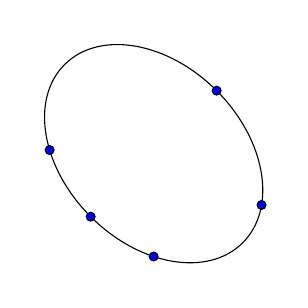
\begin{tikzpicture}[scale=0.8]
\clip(-2.,-2.) rectangle (2.,2.);
\draw [rotate around={-45.:(0.,0.)}] (0.,0.) ellipse (2.cm and 1.4142135623730951cm);
\begin{scriptsize}
\filldraw [fill=blue] (1.,1.) circle (2pt);
\filldraw [fill=blue] (-1.,-1.) circle (2pt);
\filldraw [fill=blue] (0.,-1.6329931618554518) circle (2pt);
\filldraw [fill=blue] (-1.651267157575746,0.05752458323349807) circle (2pt);
\filldraw [fill=blue] (1.7127137631328755,-0.814236214326387) circle (2pt);
\end{scriptsize}
\end{tikzpicture}
\end{figure}

The idea is that ``conics are parametrized by $\P^5$, and passing through a point is a degree $1$ equation in $\P^5$''.  But this might be dangerous:
\begin{itemize}
\item $\P^5$ parametrizes conics, not \emph{smooth} conics.
\item We need \emph{transversal} intersections.
\end{itemize}

For instance, the argument \emph{does not} work for  smooth conics tangent to five lines. Each tangency is a degree $2$ equation on $\P^5$, but they are not transversal (the conics of the form $\{L^2=0\}$ are ``tangent'' to all lines). 

The correct number is $1$, which may be seen by taking the \emph{dual conic} (the set of tangent lines, as a subset of ${ (\P^2) }^\ast$).

\subsection{Conservation of number}%
\label{sub:conservation_of_number}

The classical principle is called \emph{conservation of number}: if the problem has a finite numerical answer, this number is constant (or jumps to infinity).

Sadly, this does not work. Given four lines and a point in general position, there exists $1^4 \cdot 2=2$ smooth conics tangent to the lines and passing through the point (as one can show by taking the dual problem). But if the point lies in the diagonals of the quadrilateral given by the lines, then the number of smooth solutions decreases to $1$ or $0$. 

Today we will discuss strong foundations for this principle, and some applications in enumerative geometry. 

\section{Families of cycle classes}

During this section, $T$ will denote an irreducible variety of dimension $m>0$. We take $t \in T$ a regular closed point, and we denote
\[ \{t\}=\Spec \kappa(t), \qquad t\colon \{t\} \to T \] 
for the point and the inclusion.

We will use script letters (e.g. $\msc{X}, \msc{Y}$) for schemes over $T$, and the corresponding latin letters (e.g. $X_t, Y_t$) for the corresponding fibers over $t$ (as schemes over $\{t\}$). If $f\colon \msc{X} \to \msc{Y}$ is a morphism, we denote $f_t\colon X_t \to Y_t$ the map on the fibers.

\subsection{Specialization}%
\label{sub:specialization}


Let $p\colon \msc{Y} \to T, \alpha \in A_{k+m}\msc{Y}$. We define $\alpha_t \in A_k Y_t$ by
\[ \alpha_t = t^!(\alpha) \]
where $t^{!}$ is the refined Gysin homomorphism induced by
\[ \begin{tikzcd} Y_t \arrow[r] \arrow[d] & \msc{Y} \arrow[d, "p"] \\ {\{t\}} \arrow[r, "t"] & T. \end{tikzcd} \]
For instance, if $\alpha=[\msc{V}]$ and $\msc{V} \subseteq Y_t$, then ${[\msc{V}]}_t=0$. 

Here are some basic properties.
\begin{prop}\label{prop:basicprop}
\begin{enumerate}
\item If $f\colon \msc{X} \to \msc{Y}$ is proper, $\alpha \in A_{k+m}\msc{X}$, then
\[ f_{t\ast}(\alpha_t)={ (f_\ast(\alpha)) }_t \qquad \text{in }A_k(Y_t). \]

\item If $f\colon \msc{X} \to \msc{Y}$ is flat of relative dimension $n$, $\alpha \in A_{k+m}\msc{Y}$
\[ f_t^\ast(\alpha_t)={ (f^\ast(\alpha)) }_t \qquad \text{in }A_{k+n}(X_t). \]

\item If $i\colon \msc{X} \to \msc{Y}$ is a regular embedding of codimension $d$, such that $i_t\colon X_t \to Y_t$ is also a regular embedding of codimension $d$, $f\colon \msc{V} \to \msc{Y}$ a morphism, $\alpha \in A_{k+m}\msc{V}$, then
\[ i_t^!(\alpha_t)={ (i^!(\alpha)) }_t \qquad \text{in } A_{k-d}(W_t), \msc{W}=f^{-1}(\msc{X}). \]
\end{enumerate}
\begin{enumerate} \setcounter{enumi}{3}
\item If $E$ is a vector bundle over $\msc{Y}$, $\alpha \in A_{k+m} \msc{Y}$, then 
\[ c_i(E_t) \cap \alpha_t = { (c_i(E) \cap \alpha) }_t \qquad \text{in }A_{k-i}(Y_t). \]
\end{enumerate}
\end{prop}

The proof follows directly from similar statements for the refined Gysin homomorphism (see \textsection~6.2--6.4).

We would now like to relate different fibers. Given a family $\msc{X} \to T$ and $\alpha \in A_{k+m}\msc{X}$, it is natural to compare $\alpha_t \in A_k(X_t)$ for different values of $t$. It is not obvious that such relation exists, even if $\msc{X}=Y \times T$ is the trivial family.

\begin{exm}
Let $Y=T$ be a projective curve of genus $g \geq 2$, and $\Delta\subseteq Y \times T$ the diagonal. If $\alpha = [\Delta] \in A_1(Y \times T)$, then $\alpha_t = [t] \in A_0 Y$. But for $t_1 \neq t_2$, we have that $\alpha_{t_1}$ and $\alpha_{t_2}$ are not rationally equivalent. 
\end{exm}

This can be solved if we assume that $\msc{X}=Y \times T$, and if for every $t_1, t_2 \in T$, they can be connected by a chain of rational curves in $T$ (see Example 10.1.7).

Here is a useful corollary.
\begin{cor}\label{cor:intfiber}
Assume $T$ is non-singular, $t \in T$ rational over the ground field, $\msc{Y}$ smooth over $T$ with relative dimension $n$. If $\alpha \in A_{k+m}(\msc{Y}), \beta \in A_{l+m}(\msc{Y})$, then 
\[ \alpha_t \cdot \beta_t = { (\alpha \cdot \beta) }_t \qquad \text{in } A_{k+l-n}(Y_t). \]
\end{cor}

This gives us a strategy to show that $a \cdot b=c$ in a non-singular variety $Y$. We construct a family $\msc{Y} \to T$ with $Y_t=Y$ for some $t$, and such that $a, b, c$ can be lifted to $\alpha, \beta, \gamma$. Then, it suffices to show that $\alpha \cdot \beta=\gamma$, which we can try to prove generically.

\subsection{Sample Application}%
\label{sub:sample_application}


Let $C$ be a non-singular curve, $C^{(n)}$ its $n^{\text{th}}$ symmetric product (which points are effective divisors of degree $n$ over $C$). If $A$ is an effective divisor on $C$ of degree $<n$, define
\[ X_A=\{D \in C^{(n)} \mid D \geq A \}. \]

One can show that if $A$ and $B$ have disjoint support, then $X_A$ and $X_B$ intersect transversally, and so
\[ [X_A] \cdot [X_B]=[X_{A+B}]. \]

This is true even if $A$ and $B$ intersect, by using Corollary~\ref{cor:intfiber} and by ``moving'' $A$. 

\section{Conservation of number}

We have seen that for $\alpha \in A_k\msc{Y}$, it is not clear that ${\{\alpha_t\}}_{t \in T}$ are related, even if $\msc{Y}=Y \times T$ is the trivial family.  We have the following substitute.

\begin{prop}[Conservation of number]
Let $p\colon \msc{Y} \to T$ be a proper morphism, $\dim T=m$ as before. Let $\alpha$ be an $m$-cycle on $\msc{Y}$. Then $\alpha_t \in A_0(Y_t)$ all have the same degree (which is obtained by $p_{t\ast}(\alpha_t)=\deg \alpha_t\cdot [\{t\}]$). 
\end{prop}

The idea of the proof is write $p_\ast(\alpha)=N[T] \in A_m(T)$, for some $N \in \Z$. Then, by Proposition~\ref{prop:basicprop} we get
\[ p_{t\ast}(\alpha_t)={ (p_\ast(\alpha)) }_t = { N[T] }_t= N[\{t\}]. \]

This proposition can be improved to compute the degree of intersections with Chern classes or some divisors (see \textsection~10.2 for precise statements). We will need the following result.

\begin{cor}
Let $Y$ be a scheme, $\msc{H}_i \subseteq Y \times T$ effective Cartier divisors which are flat over $T, i=1, \dots, d$. Let $a$ be a $d$-cycle on $Y$. Assume that
\[ \msc{H}_1 \cap \dots \cap \msc{H}_d \cap (\Supp(a) \times T) \]
is proper over $T$. Then
\[ \deg({ (H_1) }_t \cdots { (H_d) }_t \cdot a) \]
is independent of $t$. 
\end{cor}

\section{An enumerative problem}

Our main application of these techniques will be to solve the following problem.
\begin{center}
\emph{Given an $r$-dimensional family of plane curves, and $r$ curves in general position in the plane, how many curves in the family are tangent to the $r$ given curves?}
\end{center}

The answer will require to compute the \emph{characteristics} $\mu^k \nu^{r-k}$ of the family, which are the number of curves in the family passing through $k$ general points and tangent to $r-k$ general lines. 

For instance, if we consider the family of smooth conics, then
\[ \mu^5 = \nu^5 = 1, \quad \mu\nu^4=\mu^4\nu=2, \quad \mu^2\nu^3=\mu^3\nu^2=4. \]

\begin{enumerate}
    \item We will study the \emph{incidence correspondence} 
\[ I=\{[x:y:z], [a:b:c] \mid ax+by+cz=0\} \subseteq \P^2 \times \P^{2\ast}. \]
This can be seen as a $\P^1$-bundle over $\P^2$. In fact, if $E$ is the kernel of
\[ 1_{\P^2}^{\oplus 3} \xrightarrow{(x, y, z)} \msc{O}_{\P^2}(1) \to 0, \]
then $I=\P(E)$. 

This allows us to compute $A^\bullet(I)$ (see Example 8.3.4), with a basis 
\[ 1, \lambda, \zeta, \lambda^2, \zeta^2, \lambda^2\zeta=\lambda\zeta^2, \]
where $\lambda\zeta=\lambda^2+\zeta^2, \lambda^3=\zeta^3=0$, and $\lambda, \zeta$ the pullbacks of $c_1(\msc{O}_{\P^2}(1)), c_1(\msc{O}_{\P^{2\ast}}(1))$. 

Now, if $M$ is a line and $Q$ a point, consider
\begin{align*}
M' &= \{(P, L) \in I \mid L=M\} & Q' &= \{(P, L) \in I \mid P=Q\} \\
M'' &= \{(P, L) \in I \mid P \in M\} & Q'' &= \{(P, L) \in I \mid Q \in L\}.
\end{align*}
One can show that
\[ \lambda=[M''], \quad \zeta = [Q''], \qquad \lambda^2=[Q'], \quad \zeta^2 = [M']. \]
    \item Let $D \subseteq \P^2$ be a curve without multiple components. Define $D' \subseteq I$ as the closure of
\[ \{(P, L) \in I \mid P \text{ simple point of D}, L \text{ tangent at }P\}. \]

We claim that
\[ [D'] = n[M']+m[Q'] = n\zeta^2+m \lambda^2 \in A^2I, \]
where $n$ is the degree and $m$ the \emph{class} of $D$ (the number of tangents from a general point to $D$). The idea is to compute 
\[ D' \cap M'' = \{(P_i, L_i) \mid P_i \in M \cap D, L_i \text{ tangent at }P_i\}, \]
which has generically $\# D' \cap M''=n$ points.  

The equivalence $[D']=m[M']+n[Q']$ can be computed explicitely. Take $P_0$ a general point, $M$ a general line, and let $Q_1, \dots, Q_m$ the intersections of $M$ with the tangents from $P_0$.
\begin{figure}[H]
\centering
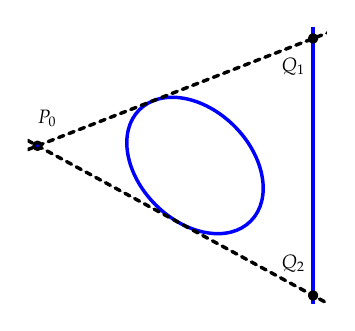
\begin{tikzpicture}[scale=0.5, line cap=round,line join=round, line width=1.25pt]
\clip(-4.25,-3.5) rectangle (3.35,3.5);
\draw [rotate around={-45.:(0.,0.)},color=blue] (0.,0.) ellipse (2.cm and 1.4142135623730951cm);
\draw [color=blue] (3.,-3.5) -- (3.,3.5);
\draw [dash pattern=on 2pt off 2pt,domain=-4.25:3.35] plot(\x,{(-6.062177826491071-1.9684926258021747*\x)/3.6235853534352556});
\draw [dash pattern=on 2pt off 2pt,domain=-4.25:3.35] plot(\x,{(--6.0621778264910695--1.1472635755228446*\x)/2.9462470487993815});
\begin{scriptsize}
\draw [fill=blue] (-4.,0.5) circle (2.5pt);
\draw [fill=black] (3.,3.2257880604182683) circle (2.5pt);
\draw [fill=black] (3.,-3.3027111373413454) circle (2.5pt);
\draw (-3.75, 1.2) node {$P_0$};
\draw (2.5,2.5) node {$Q_1$};
\draw (2.5,-2.5) node {$Q_2$};
\end{scriptsize}
\end{tikzpicture}
\end{figure}

The projection from $P_0$ to $M$ gives a family $\mathscr{D} \to \mathbb{A}^1$ with $\mathscr{D}_1=[D'], \mathscr{D}_0 = n[M']+\sum [Q_i']$. (There is a explicit computation in \textsection~10.4.) 
    \item Let $\mathscr{X} \subseteq \P^2 \times S$ be a flat family of plane curves, $\dim S=r$, $S$ non-singular. Assume $X_s$ has no multiple compontents for general $s$, and let $S^0 \subseteq S$ an open set with $X_s$ reduced for $s \in S$. 

Let $\msc{X}(r)\subseteq I^r \times S^0$ given by $(P_1, L_1), \dots, (P_r, L_r), s$ such that $P_i$ is a simple point of $X_s$, and $L_i$ is tangent in $P_i$. Note that $\dim \msc{X}(r)=2r$.

Take $D_1, \dots, D_r \subseteq \P^2$ reduced curves, and consider
\[ \begin{tikzcd} W \arrow[r] \arrow[d] & D_1' \times \cdots \times D_r' \arrow[d] \\ \msc{X}(r) \arrow[r, "\varphi"] & I^r. \end{tikzcd} \]

We can move $D_1, \dots, D_r$, so that the interseccion between $\msc{X}(r)$ and $D_1' \times \cdots \times D_r'$ is transversal (by taking a general element in ${ \operatorname{PGL}(2) }^r$). This way, $W$ has $N$ (reduced) points. 

Now, compactify $\overline{\msc{X}} \subseteq \P^2 \times \overline{S^0}$, and $\overline{\msc{X}(r)}\subseteq I^r \times \overline{S^0}$. If $Z$ is a closed subsed of dimension less than $2r$, which contains all $\overline{\msc{X}(r)}-\msc{X}(r)$, then the number $N$ does not change after we remove $Z$.
    \item We now degenerate each $D_i$ to a multiple line (as we did for $D$). This gives a diagram
\[ \begin{tikzcd} \msc{W} \arrow[r] \arrow[d] & \msc{D}_1' \times \cdots \times \msc{D}_r' \arrow[r] \arrow[d] & \A^r \\ \overline{\msc{X}(r)} \arrow[r]& I^r. \end{tikzcd} \]
The space $\overline{\msc{X}(r)}$ is complete, so $\msc{W}$ is proper over $\A^r$. This way, we may take an open neighborhood $T$ of $(1, \dots, 1)$ and $(0, \dots, 0)$, so that $\msc{W}$ is proper over $T$ and disjoint from $Z$. 

Now, Corollary~\ref{cor:intfiber} applies, and so
\[ \deg(\msc{X}(r) \cdot_\varphi (D_1' \times \cdots \times D_r')) = \deg(\msc{X}(r) \cdot_\varphi (E_1' \times \dots E_r')), \]
where $D_i', E_i'$ are the fibers over $1$ and $0$.

The right hand side is just
\[ \prod_{i=1}^r (m_i \mu + n_i \nu) = \sum_{k=0}^r N_k \mu^k \nu^{r-k}, \]
where each curve $D_i$ has degree $n_i$ and class $m_i$. 

The left hand side is the number of points $N$, provided that we take a \emph{convenient} $Z$ (which avoids technical difficulties such as bitangents). 
\end{enumerate}

\subsection{A famous example}%
\label{sub:a_famous_example}

The most famous example is the \emph{Steiner's conic problem}, which tries to determine the number of conics tangent to five smooth conics in general position. 

The natural family here is the family of smooth conics (as a subset of $\P^5$), which has characteristics
\[ \mu^5=\nu^5=1, \quad \mu^4\nu=\mu\nu^4=2, \mu^3\nu^2=\mu^2\nu^3=4 \]
(in characteristic zero!)

This way, the number of conics tangent to five non-singular curves of degree $n$ in general position is
\[ N=n^5({ (n-1) }^5+10{ (n-1) }^4+40{ (n-1) }^3+40{ (n-1) }^2+10(n-1)+1), \]
which for $n=2$ gives the famous number $3264$. 

\chapter{Patrick (Mar 19): Doing Italian-style algebraic geometry rigorously}%
\label{cha:patrick_mar_19_doing_italian_style_algebraic_geometry_rigorously}

\textit{Note: these are the speaker's notes.} 

\section{Intersection multiplicities}%
\label{sec:intersection_multiplicities}

Consider a Cartesian square
\begin{equation*}
\begin{tikzcd}
    W \ar{r}{j} \ar{d}{g} & V \ar{d}{f} \\
    X \ar{r}{i} & Y
\end{tikzcd}
\end{equation*}
where $i$ is a regular embedding of codimension $d$ and $V$ has pure dimension $k$. Let $C = C_W V$ have components $C_1, \ldots, C_r$ with multiplicity $m_i$. Let $Z_i$ be the support of $C_i$. We call the $Z_i$ the \textit{distinguished varieties} of the intersection.

\begin{lem}\leavevmode
    \begin{enumerate}[(a)]
        \item Every irreducible component of $W$ is distinguished.
        \item For any distinguished variety $Z$, we have $k-d \leq \dim Z \leq k$.
    \end{enumerate}
\end{lem}

\begin{defn}
    An irreducible component $Z$ of $W = f^{-1}(X)$ is a \textit{proper component} of intersection of $V$ by $X$ if $\dim Z = k-d$. The \textit{intersection multiplicity} of $Z$ in $X \cdot V$, denoted $i(Z, X \cdot V; Y) = i(Z, X \cdot V) = i(Z)$ is the coefficient of $Z$ in the class $X \cdot V \in A_{k-d}(W)$. 
\end{defn}

If $N_Z$ is the pullback of $N_X Y$ to $Z$, then $i(Z,X\cdot V; Y)$ is the coefficient of $N_Z$ in $[C]$. Now let $A = \msc{O}_{Z,V}$ and $J \subset A$ be the ideal of $W$. Then $A/J$ has finite length when $Z$ is an irreducible component of $W$.

\begin{prop}
    Assume $Z$ is a proper component of $W$.
    \begin{enumerate}[(a)]
        \item If $\ell(A/J)$ is the length of $A/J$, then $1 \leq i(Z, X \cdot V; Y) \leq \ell(A/J)$.
        \item If $J$ is generated by a regular sequence of length $d$, then $i(Z, X \cdot V; Y) = \ell(A/J)$.
    \end{enumerate}
    If $A$ is Cohen-Macaulay, then local equations for $X$ in $Y$ give a regular sequence generating $J$ and equality in (b) holds.
\end{prop}

Now suppose $Z$ is a proper component of the intersection of $V$ by $X$ on $Y$. Let $A = \msc{O}_{V,Z}$ and $J$ be the ideal in $A$ generated by the ideal (sheaf) of $X$ in $Y$, and let $\mf{m}$ be the maximal ideal of $A$.

\begin{prop}
    Suppose $V$ is a variety. Then $i(Z, X \cdot V; Y) = 1$ if and only if $A$ is regular and $J = \mf{m}$.
\end{prop}

\section{Nonsingular varieties}%
\label{sec:nonsingular_varieties}

Let $Y$ be a smooth variety of dimension $n$. Then $\Delta \subset Y \times Y$ is regularly embedded with codimension $n$. The global \textit{intersection product} is the map 
\[ A_k(Y) \otimes A_{\ell}(Y) \to A_{k+\ell-n}(Y) \qquad x \otimes y \mapsto x \cdot y \Delta^*(x \times y), \] 
where $\delta^*$ is the Gysin homomorphism.

More generally, let $X$ be a scheme and $f \colon X \to Y$ a morphism to a smooth variety. Then $\Gamma_f$ is regularly embedded in $Y$, so we can define a \textit{cap product}
\[ A_i (Y) \otimes A_j (X) \to A_{i+j-n}(X) \qquad y \otimes x \mapsto f^*(y) \cap x = \Gamma_f^*(x \times y). \]
If $X$ is smooth, then we write $f^*y = f^* y \cap [X]$.

\begin{rmk}
    We may also replace the Gysin homomorphisms $\Delta^*, \Gamma_f^*$ with the refined Gysin homomorphisms $\Delta^{!}, \Gamma_f^{!}$.
\end{rmk}

\begin{defn}
    Let $f \colon X \to Y$ be a morphism with $Y$ smooth of dimension $n$. Let $p_X \colon X' \to X, p_Y \colon Y' \to Y$ be morphisms of schemes. Then form the square
    \begin{equation*}
    \begin{tikzcd}
        X' \times_Y Y' \ar{d} \ar{r} & X' \times Y' \ar{d}{p_X \times p_Y} \\
        X \ar{r}{\Gamma_f} & X \times Y.
    \end{tikzcd}
    \end{equation*}
    Now define the \textit{refined intersection product} by
    \[ x \cdot_f y \coloneqq \Gamma_f^{!} (x \times y) \in A_{k+\ell-n}(X' \times_Y Y') \]
    for $x \in A_k(X'), Y \in A_{\ell}(Y')$. When $X' = X, Y' = Y$, this is the global product.
\end{defn}

\begin{prop}
    The refined products satisfy the following formal properties:
    \begin{enumerate}[(a)]
        \item (Associativity) If $X \xrightarrow{f} Y \xrightarrow{g} Z$ with $Y, Z$ smooth, then 
            \[ x \cdot_f (y \cdot_g z) = (x \cdot_f y) \cdot_{gf} z \in A_*(X' \times_Y Y' \times_Z Z'). \]
        \item (Commutativity) If $f_i \colon X \to Y_i$ with $Y_i$ smooth, then
            \[ (x \cdot_{f_1} y_1) \cdot_{f_2} y_2 = (x \cdot_{f_2} y_2) \cdot_{f_1} y_1 \in A_*(Y'_1 \times_{Y_1} X' \times_{Y_2} Y_2'). \]
        \item (Projection) Let $X \xrightarrow{f} Y \xrightarrow{g} Z$ with $Z$ smooth. Let $f' \colon X' \to Y'$ be proper with $p_Y f' = f p_X$ and $f'' = f' \times_Z \mr{id}_Z$. Then
            \[ f''_* (x \times_{gf} z) = f'_*(x) \cdot_g z \in A_*(Y' \times_Z Z'). \]
        \item (Compatibility) Let $f \colon X \to Y$ with $Y$ smooth and $g \colon V' \to Y'$ be a regular embedding. Then 
            \[ g^{!}(x \cdot_f y) = x \cdot_f g^{!}y \in A_*(X' \times_Y V'). \]
    \end{enumerate}
\end{prop}

\begin{cor}
    Let $Y$ be smooth and $j \colon V \to Y$ be a regular embedding. If $x$ is a cycle on $Y$, then $x \cdot [V] = j^!(x) \in A_*(\abs{x} \cap V)$.
\end{cor}

\begin{cor}
    Let $f \colon X \to Y$ with $X,Y$ smooth. Then $x \cdot_f y = (x \times y) \cdot [\Gamma_f] \in A_*(\abs{x} \cap f^{-1}(\abs{y}))$.
\end{cor}

\begin{cor}
    Let $f \colon X \to Y$ with $Y$ smooth and $x$ a cycle on $X$. Then $x \cdot_f [Y] = x$.
\end{cor}

\begin{defn}
    Let $f \colon X \to Y$ be a morphism with $X$ purely $m$-dimensional and $Y$ a smooth $n$-dimensional variety $Y$. For any morphism $g \colon Y' \to Y$, define a \textit{refined Gysin homomorphism}
    \[ f^{!} \colon A_k(Y') \to A_{k+m-n}(X \times_Y Y') \qquad f^!(y) = [X] \cdot_f y. \]
\end{defn}

\begin{prop}\leavevmode
    \begin{enumerate}[(a)]
        \item If $f$ is flat, then $f^!(y) = f'^*(y)$, where $f' \colon X \times_Y Y' \to Y'$ is the base change.
        \item If $f$ is a local complete intersection morphism, then $f^{!}$ agrees with the morphism constructed in Section 6.6 of Fulton.
    \end{enumerate}
\end{prop}

Now let $Y$ be a smooth variety of dimension $n$. Let $V, W$ be closed subschemes of $Y$ of pure dimension $k, \ell$. Now a component $Z \subseteq V \cap W$ is a \textit{proper component} if $\dim Z = k + \ell - n$. If $Z$ is proper, then the coefficient of $Z$ in $V \cdot W \in A_{k+\ell-n}(V \cap W)$ is called the \textit{intersection multiplicity} $i(Z, V \cdot W; Y) = i(Z, \Delta_Y \cdot (V \times W); Y \times Y)$. If every component of $V \cap W$ is proper, then the intersection class is
\[ V \cdot W = \sum_Z i(Z, V \cdot W; Y) \cdot [Z]. \]
\begin{prop}
    Assume $Z$ is a proper component of $V \cap W$. Then
    \begin{enumerate}[(a)]
        \item $1 \leq i(Z, V \cdot W; Y) \leq \msc{O}_{V \cap W, Z}$.
        \item If the local ring $\msc{O}_{V \cap W, Z}$ is Cohen-Macaulay, then $i(Z,V \cdot W; Y) = \ell(\msc{O}_{V \cap W, Z})$.
        \item If $V, W$ are varieties, then $i(Z, V \cdot W; Y) = 1$ if and only if the maximal ideal of $\msc{O}_{Y,Z}$ is the sum of the prime ideals of $V$ and $W$. In fact, $\msc{O}_{V,Z}, \msc{O}_{W,Z}$ are regular.
    \end{enumerate}
\end{prop}

Now let $Y$ be a smooth variety of dimension $n$. Set $A^p(Y) = A_{n-p}(Y)$. Now this indexing, the intersection product is now $A^p(Y) \otimes A^q(Y) \to A^{p + q}(Y)$. In addition, if $f \colon X \to Y$ is a morphism, the cap product is now $A^p(Y) \otimes A_q(X) \xrightarrow{\cap} A_{q-p}(X)$. If $X$ is also smooth, the pullback now reads $f^* \colon A^p(Y) \to A^p(X)$. 

\begin{prop}\leavevmode
    \begin{enumerate}[(a)]
        \item Suppose $Y$ is a smooth variety. Then the intersection product makes $A^*(Y)$ into a commutative graded ring with unit $A^0 \ni 1 = [Y] \in A_n$. Then $Y \mapsto A^*(Y)$ is a contravariant functor from smooth varieties to rings.
        \item If $f \colon X \to Y$ is a morphism from a scheme $X$ to a smooth variety $Y$, then $A_* X$ is a $A^* Y$-module with action
            \[ A^p(Y) \otimes A_q(X) \xrightarrow{\cap} A_{q-p}(X). \]
        \item If $f \colon X \to Y$ is a proper morphism of smooth varieties, then
            \[ f_* (f^*y \cdot x) = y \cdot f_*(x) \]
            for all classes $x$ on $X$ and $y$ on $Y$.
    \end{enumerate}
\end{prop}

\section{B\'ezout's Theorem}%
\label{sec:bezout_s_theorem}

We will now use this theory to discuss something classical. It is easy to see that $A_k(\P^n) \cong \Z$ and is generated by $[L^k]$ for a linear subspace $L^k \subset \P^n$. If $\alpha$ is a $k$-cycle on $\P^n$, we define the \textit{degree} $\deg (\alpha)$ to be the integer satisfying $\alpha = \deg (\alpha) \cdot [L^k]$. Equivalently, we may define
\[ \deg(\alpha) = \int_{\P^n} {c_1(\msc{O}(1))}^k \cap \alpha. \]

\begin{thm}[B\'ezout]
    Let $\alpha_i \in A^{d_i}(\P^n)$ for $i = 1, \ldots, r$. If $d_1 + \cdots + d_r \leq n$, then
    \[ \deg(\alpha_1 \cdots \alpha_r) = \deg(\alpha_1) \cdots \deg(\alpha_r). \]
\end{thm}

\begin{proof}
    We have an isomorphism $A^*(\P^n) = \Z[h]/(h^{n+1})$, where $h = [L^{n-1}]$. Thus $[L^{n-k}] = h^k$, and the desired result follows.
\end{proof}

Now if subschemes $V_1, \ldots, V_r \subseteq \P^n$ representing $\alpha_1, \ldots, \alpha_r$ meet properly, then 
\[ V_1 \cdots V_r = \sum_j i(Z_j, V_1 \cdots V_r; \P^n) \cdot [Z_j], \]
where $Z_j$ are the components of $\bigcap V_i$. Then B\'ezout's theorem gives us the identity
\[ \sum_j i(Z_j, V_1 \cdots V_r; \P^n) \cdot \deg(Z_j) = \prod \deg(V_i). \]
If $H_1, \ldots, H_n$ are hypersurfaces intersecting properly (so the intersection is a finite number of points), then consider the local ring $\msc{O}_{\bigcap H_i,P}$. Then complete intersections are Cohen-Macaulay, so 
\[ i(P, H_1 \cdots H_n; \P^n) = \ell(\msc{O}_{\bigcap H_i, P}). \]
Now $\dim_k \msc{O}_{\bigcap H_i, P} = \deg P \ell(\msc{O}_{\bigcap H_i, P})$, and thus we obtain
\[ \sum_P \dim_k \msc{O}_{\bigcap H_i, P} = \prod \deg H_i. \]
This recovers the very classical B\'ezout's theorem.

\begin{exm}
    Let $s$ be the hyperplane class on $\P^n$ and $t$ be the hyperplane class on $\P^m$. Then 
    \begin{enumerate}
        \item $A^*(\P^n \times \P^m) = \Z[s,t]/(s^{n+1}, t^{m+1})$.
        \item If $H_1, \ldots, H_{n+m}$ are hypersurfaces in $\P^n \times \P^m$ with bidegree $(a_i, b_i)$, then
            \[ \int [H_1] \cdots [H_{n+m}] = \sum_{ \substack{(i_1, \ldots, i_n, j_1, \ldots, j_m) \\ (n,m)\text{-shuffle}} } a_{i_1} \cdots a_{i_n} b_{j_1} \cdots b_{j_m}. \]
        \item If $\Delta$ is the diagonal in $\P^n \times \P^n$, then $[\Delta] = \sum_{i=0}^n s^i t^{n-i} \in A^n(\P^n \times \P^n)$. 
            This formula follows from intersecting $\Delta$ with $[L_1 \times L_2]$, where $L_1, L_2$ are linear subspaces of complementary dimension.
        \item Let $s \colon \P^n \times \P^m \to \P^{nm+n+m}$ be the Segre embedding. It $h$ is the hyperplane class on $\P^{nm+n+m}$, then $s^* u = s + t$. Also, the degree of $s(\P^n \times \P^m)$ is $\binom{n+m}{n}$.
        \item If $v_m \colon \P^n \to \P^{\binom{n+m}{n}-1}$ is the Veronese embedding and $s,h$ are the hyperplane classes on the source and target, then $v_m^* u = m \cdot s$. If $V$ is a $k$-dimensional subvarity of $\P^n$ of degree $d$, then $\deg(v_m(V)) = d \cdot m^k$.
    \end{enumerate}
\end{exm}

\chapter{Morena (Mar 26): Grothendieck-Riemann-Roch}%
\label{cha:morena_mar_26_grothendieck_riemann_roch}

We will begin by reviewing some notions from algebraic topology. 
\begin{enumerate}
    \item Let $E$ be a vector bundle over $X$ with Chern roots $\alpha_1, \ldots, \alpha_r$. Then we may define the \textit{Chern character} 
        \[ \ch(E) = \sum_{i=1}^r e^{\alpha_i} = \sum_{n=0}^{\infty} \frac{s_n(c_1, \ldots, c_n)}{n!}, \]
        where $s_n$ is the $n$-th Newton polynomial. Recall that if
        \[ 0 \to E' \to E \to E'' \to 0 \]
        is exact, then $\ch(E) = \ch(E') + \ch(E'')$ and $\ch(E \otimes F) = \ch(E) \ch(F)$.
    \item We may define the \textit{Todd class}
        \[ \td(E) = \prod_{i=1}^r \frac{\alpha_i}{1-e^{-\alpha_i}}. \]
        Similarly to Chern classes, if 
        \[ 0 \to E' \to E \to E'' \to 0 \]
        is exact, then $\td(E) = \td(E') \td(E'')$.
    \item Now define the ring
        \[ K^0(X) = \bigoplus \Z[E] / (0 \to E' \to E \to E'' \to 0). \]
        This is well-behaved under pullback, but pushforward is not well-defined. 
\end{enumerate}

In order to fix the problems with pushforwards of vector bundles, we will attempt to define the Grothendieck group $K_0(X)$ of coherent sheaves. Unfortunately, pullbacks of coherent sheaves are only right exacts. Also, pushforwards do exist for proper morphisms, but this is only left exact. Therefore we need to consider the higher derived functors, and now we define
\[ f_* \colon K_0(X) \to K_0(Y) \qquad [\msc{F}] \mapsto \sum_{i=0}^{\infty} {(-1)}^i [R^i f_* \msc{F}]. \]
This is a finite sum because we assume all of our schemes are Noetherian.

For a smooth variety, there is always a map $K^0(X) \to K_0(X)$. In fact, there is an inverse, because we can resolve any coherent sheaf $\msc{F}$ by vector bundles. In this case, we will write $K_0(X) = K^0(X) = K(X)$. If $\msc{F}$ is resolved by
\[ 0 \to \msc{L}_n \to \cdots \to \msc{L}_0 \to \msc{F} \to 0, \]
we write $[\msc{F}] = \sum_{i=0}^n [\msc{L}_i]$ and $\ch(\msc{F}) = \sum_{i=0}^n {(-1)}^i \ch(\msc{L}_i)$.

\section{Statement of the theorem}%
\label{sec:statement_of_the_theorem}

Recall the Chern character $\ch \colon K(X) \to A(X) \otimes \Q$. In topology, we need the Todd class to make the diagram
\begin{equation*}
\begin{tikzcd}
    K(X) \ar{r}{\lambda_E} \ar{d}{\ch} & K(E) \ar{d}{\ch \cdot {(-1)}^{\mr{rk}(E)} \td(E^*)} \\
    H^*(X, \Q) \ar{r}{u_E} & H^*(X, \Q)
\end{tikzcd}
\end{equation*}
commute. Now we are able to state the Grothendieck-Riemann-Roch theorem:

\begin{thm}[Grothendieck-Riemann-Roch]
    Let $f \colon X \to Y$ be proper where $X, Y$ are smooth quasiprojective varieties over $k$. Then the diagram
    \begin{equation*}
    \begin{tikzcd}
        K(X) \ar{r}{f_*} \ar{d}{\ch \cdot \td(T_X)} & K(Y) \ar{d}{\ch \cdot \td(T_Y)} \\
        {A(X)}_{\Q} \ar{r}{f_*} & {A(Y)}_{\Q}
    \end{tikzcd}
    \end{equation*}
    commutes. In other words, $f_*(\ch(-) \cdot \td(T_X)) = \ch(f_*(-)) \cdot \td(T_Y)$.
\end{thm}

First, we will see why this implies the classical (Hirzebruch)-Riemann-Roch theorem. First, let $X$ be a curve, $Y = \mr{pt}$, and $\msc{L}$ be a line bundle. Then the right hand side is 
\[ \ch(f_* [\msc{L}]) = {(-1)}^i H^i(X, \msc{L}) = \chi(X, \msc{L}). \]
On the other side, we have
\begin{align*}
    f_* (1 + c_1(\msc{L})) ( 1 + c_1(T_X)/2 ) &= f_*(c_1(\msc{L}) + c_1(\msc{T_X})/2) \\
                                              &= \deg(\msc{L}) - \frac{1}{2} \deg(K) \\
                                              &= \deg(\msc{L}) - g + 1.
\end{align*}
This recovers the classical Riemann-Roch theorem.

Now let $X$ be a smooth surface. Then our formula becomes
\begin{align*}
    \chi(X, \msc{L}) &= f_* \qty( \qty(1 + c_1(\msc{L} + \frac{c_1^2(\msc{L})}{2})) \qty(1 + \frac{c_1(T_X)}{2} + \frac{c_1^2(TX) + c_2(TX)}{2}) ) \\
                     &= \deg \qty( \frac{c_1^2(\msc{L})}{2} - \frac{c_1(\msc{L}) c_1(\Omega_X)}{2} + \frac{c_1^2(\Omega_X) - c_2(\Omega_X)}{12} ). 
\end{align*} 
This recovers the Hirzebruch-Riemann-Roch theorem.

\section{Proof for $\P^m \to \mr{pt}$}%
\label{sec:proof_for_p_m_to_pt_}

First, we have the following theorem:
\begin{thm}
    $K(\P^m)$ is generated by $[\msc{O}_{\P^m}(n)]$ for $0 \leq n \leq m$.
\end{thm}

To prove this, we need to find a resolution of a coherent sheaf $\msc{F}$ by line bundles, so we have
\[ 0 \to \bigoplus \msc{L_i}^{(n)} \to \cdots \to \bigoplus \msc{L}_i^{(0)} \to \msc{F} \to 0. \]
Because $\msc{O}(1)$ is ample, $\msc{F} \otimes \msc{O}(N)$ is generated by global sections, so we have the exact sequence
\[ 0 \to \cdots \to \bigoplus \msc{O} \to \msc{F} \otimes \msc{O}(N) \to 0, \]
and we can tensor this by $\msc{O}(-N)$. Now if we set $V = \bigoplus^{m+1} \msc{O}(-1)$, we can take the Koszul complex
\[ 0 \to {\bigwedge}^{m+1} V \to \cdots \to {\bigwedge}^0 V \to 0. \]
Now we have the exact sequence
\[ 0 \to \msc{O}(-m-1) \to \cdots \to \bigoplus \msc{O}(-m-1+j) \to \cdots \to \msc{O} \to 0. \]
In particular, this means that we can generate $K(\P^m)$ by $\qty{\msc{O}, \msc{O}(1), \ldots, \msc{O}(m)}$.

Now it remains to prove Grothendieck-Riemann-Roch just for $\msc{O}(n), 0 \leq n \leq m$. Here, because $Y$ is a point, we have $\ch(f_*(-)) \td(T_*) = \chi(X, -)$. In our case, we know that for $0 < i < m$, $H^i(\P^m, \msc{O}(n)) = 0$ and $H^m(\P^m, \msc{O}(n)) = {H^0(\P^n, \msc{O}(-n-m-1))}^{\vee} = 0$, so
\[ \chi(\P^n, \msc{O}(n)) = h^n(\P^n, \msc{O}(n)) = \binom{n+m}{m} \]
by basic combinatorics.\footnote{If you are unsure of this, this is an exercise in Giulia's homework. If you need a hint, please email Caleb, who has several publications in combinatorics, at \url{calebji@math.columbia.edu}.}

On the other hand, we want to compute $f_*(\ch(\msc{O}(n)) \td(T_{\P^m}))$. Recall the Euler exact sequence
\[ 0 \to \msc{O} \to {\msc{O}(1)}^{\oplus m+1} \to T_{\P^m} \to 0. \]
Therefore we have $\td(T_{ \P^m }) = { \td(\msc{O}_{\P^n}) }^{m+1}$. Also, $\ch(\msc{O}(n)) = { \ch(\msc{O}(1)) }^n = e^{xn}$. Looking for the $x^m$-coefficient in $\frac{e^{xn} x^{m+1}}{{(1-e^{-x})}^{m+1}}$, we can multiply by $x^{m+1}$ and compute the residue to obtain $\binom{m+n}{n}$.

\begin{rmk}
    Grothendieck allegedly said the following\footnote{This is supposedly translated from German, but I am unsure of the quality of the translation.} about this result:
    \begin{quotation}
        \textit{I would need to misuse about 2h of my listener's time in order to impart only an approximal understanding of this statement for $f \colon X \to Y$. In cold print (as in Springer's lecture notes) this would take around 400-500 pages. A thrilling example of how our urge for knowledge and discoveries decays into a lifeless and ideological delirium while life itself goes thousandfold to the devil -- and is threatened with final destruction. It's high time to change our course!} 
    \end{quotation}
\end{rmk}
















\end{document}
